\chapter{Sensitivity of Density Estimators via Influence Functions}
\label{ch5}


From numerical examples and discussions in Chapter \ref{ch4}, we have seen that the regularized SM density estimates with and without the presence of an isolated observation can be very different. This motivates us to study the sensitivity of the density estimators to the input data. The tool we use an extension of the classic influence function. 

We will give a review of the influence function and its applications in Section \ref{section-influence-function-review}, and then introduce our extension of this classic notion to the studies of density estimators in Section \ref{section-influence-function-extension}. We will focus on the finite-dimensional exponential family and the infinite-dimensional kernel exponential family in Sections \ref{section-influence-function-fin-dim-exp-fam} and \ref{section-influence-function-kernel-exp-fam}, respectively, and discuss various properties of the influence functions of ML and SM density projections (to be defined) in them. 

\section{A Review of Influence Function and Its Applications}\label{section-influence-function-review}

Influence function, a classical notion from robust statistics, was first introduced by \textcite{Hampel1968-gm} to investigate the infinitesimal behavior of real- and vector-valued statistical functionals and has become one of the most important tools in robust statistics \parencite{Hampel1986-ig}. 

Let $F$ be a distribution over the sample space $\calX$, and $T$ to be a statistical functional, any function of $F$. With the introduction of the statistical functional, we can express an estimator as a statistical functional evaluated at the empirical distribution function $F_n$, or, more broadly, as a function of a distribution function. This allows us to think about how the estimates were to change if we perturb the distribution function. In this section, we assume that $T$ is vector-valued so that $T \parens{F} \in \Real^m$. The \textit{influence function} of $T$ at $F$ is defined to be 
\begin{align}
	\mathrm{IF} \parens{T, F, y} := & \, \lim_{\varepsilon \to 0^+} \frac{1}{\varepsilon} \parens[\Big]{T \parens[\big]{\parens{1 - \varepsilon} F + \varepsilon \delta_y} - T \parens{F}} \label{eq-inf-fun-1} \\
	= & \, \frac{\diff}{\diff \varepsilon} T \parens[\big]{\parens{1 - \varepsilon} F + \varepsilon \delta_y} \bigg\vert_{\varepsilon=0}, \label{eq-inf-fun-2}
\end{align}
where $\delta_y$ denotes the point mass 1 at $y \in \calX$. Inspecting \eqref{eq-inf-fun-1} and \eqref{eq-inf-fun-2}, we see $\mathrm{IF} \parens{T, F, y}$ is nothing but the G{\^a}teaux derivative of the statistical functional $T$ at the distribution $F$ in the direction of the point mass $\delta_y$. Various properties of $\mathrm{IF} \parens{T, F, y}$ have been discussed by \textcite{Hampel1974-oe}, \textcite{Hampel1986-ig}, and \textcite{Wasserman2006-lj}. 

In particular, the influence function $\mathrm{IF} \parens{T, F, y}$ is a function of $y \in \calX$. It helps us understand how the estimate changes as a function of a perturbation of the data or more generally a perturbation of the assumed model, and measures the impact of an infinitesimally small amount of contamination of the original distribution $F$ at $y \in \calX$ on the quantity of interest $T \parens{F}$. 

%Then, the  is 
%\begin{align}\label{eq-gateaux-derivative}
%	\lim_{\varepsilon \to 0} \frac{1}{\varepsilon} \parens[\Big]{T \parens[\big]{\parens{1 - \varepsilon} F + \varepsilon G} - T \parens{F}}, 
%\end{align}
%which a generalization of the concept of directional derivative in the differential calculus. If we let $G = \delta_y$, the point mass 1 at $y \in \calX$, we obtain 

The \textit{empirical influence function} \parencite[Definition 2.18 in][]{Wasserman2006-lj} is defined by letting $F$ in $\mathrm{IF} \parens{T, F, y}$ be $F_n$. In addition, the \textit{sample influence function} \parencite{Hampel1974-oe, Cook1982-gj} is defined to be 
\begin{align}\label{eq-sample-inffun}
	\mathrm{SIF}_{\varepsilon} \parens{T, F_n, y} := \frac{1}{\varepsilon} \parens[\Big]{T \parens[\big]{\parens{1 - \varepsilon} F_n + \varepsilon \delta_y} - T \parens{F_n}}, 
\end{align}
where $\varepsilon > 0$ is tiny. Essentially, $\mathrm{SIF}_{\varepsilon} \parens{T, F_n, y}$ is a finite-difference approximation of $\mathrm{IF} \parens{T, F_n, y}$, and can be very useful when $T \parens{\parens{1 - \varepsilon} F_n + \varepsilon \delta_y}$ and $T \parens{F_n}$ are analytically intractable or the limit by letting $\varepsilon \to 0^+$ is hard to handle. If, in particular, we let $\varepsilon = \frac{1}{n+1}$ in \eqref{eq-sample-inffun}, we obtain Tukey's \textit{sensitivity curve} which is used to assess the sensitivity of an estimator to the position of an additional observation \emph{not} present in the sample \parencite{Hampel1986-ig}; and, if we let $\varepsilon = -\frac{1}{n-1}$ in \eqref{eq-sample-inffun}, the resulting sample influence function has a close connection with the leave-one-out cross validation and the jackknife \parencite[see Example 3.18 in][for a discussion]{Wasserman2006-lj}. 

We provide three examples below to illustrate the concept of the influence function. 

\begin{example}[Mean]\label{example-inf-fun-mean}
	Let $\calX = \Real$ and consider the statistical function defined by $T_1 \parens{F} = \int_{\Real} x \diff F \parens{x} =: \E_F \bracks{X}$, where we assume $\E_F \bracks{X}$ exists. Since 
	\begin{align*}
		\frac{1}{\varepsilon} \parens[\Big]{T_1 \parens[\big]{\parens{1 - \varepsilon} F + \varepsilon \delta_y} - T_1 \parens{F} } 
		= & \, \frac{1}{\varepsilon} \parens[\bigg]{\int_{\calX} x \diff \parens[\big]{\parens{1 - \varepsilon} F + \varepsilon \delta_y} \parens{x} - \int_{\calX} x \diff F \parens{x} } \nonumber \\ 
		= & \, \frac{1}{\varepsilon} \int_{\calX} x \diff \parens{ - \varepsilon F + \varepsilon \delta_y} \parens{x} \nonumber \\ 
		= & \, \int_{\calX} x \diff \parens{\delta_y - F} \parens{x} \\ 
		= & \, y - \E_F \bracks{X}, 
	\end{align*}
	we have 
	\begin{align}\label{eq-inf-fun-mean}
		\mathrm{IF} \parens{T_1, F, y} = y - \E_F \bracks{X}. 
	\end{align}
\end{example}

\begin{example}[Median]\label{example-inf-fun-median}
	Let $\calX = \Real$ and consider the statistical function defined by $T_2 \parens{F} = F^{-1} \parens{\frac{1}{2}}$, the median of the distribution $F$. Here, we assume $F$ has a density function $p_0$ that is symmetric around 0 and $p_0 \parens{0} \neq 0$. Then, we have $F^{-1} \parens{\frac{1}{2}} = 0$. Let $F_{\varepsilon, y} := \parens{1 - \varepsilon} F + \varepsilon \delta_y$. 
	
	First consider the case $y = 0$. Then, for any $\varepsilon \in \parens{0, 1}$, we have $F_{\varepsilon, 0} \parens{x} < \frac{1}{2} \parens{1-\varepsilon}$ for all $x < 0$ and $F_{\varepsilon, 0} \parens{x} > \frac{1}{2} \parens{1 + \varepsilon}$ for all $x > 0$. It follows that $F_{\varepsilon, 0}^{-1} \parens{\frac{1}{2}} = 0$ and $\mathrm{IF} \parens{T_2, F, 0} = 0$. 
	
	Now, suppose $y \neq 0$. We must have $\frac{1}{2} = F_{\varepsilon, y} \parens[\big]{F_{\varepsilon, y}^{-1} \parens{\frac{1}{2}}}$, which is equivalent to 
	\begin{align*}
		\frac{1}{2} = \parens{1 - \varepsilon} F \parens[\bigg]{ F_{\varepsilon, y}^{-1} \parens[\bigg]{\frac{1}{2}}} + \varepsilon \delta_y \parens[\bigg]{ F_{\varepsilon, y}^{-1} \parens[\bigg]{\frac{1}{2}}}. 
	\end{align*}
	Differentiating both sides of the preceding equation with respect to $\varepsilon$ and evaluating at $\varepsilon = 0$, we have 
	\begin{align*}
		0 = & \, - F \parens[\bigg]{ F^{-1} \parens[\bigg]{\frac{1}{2}}} + p_0 \parens[\bigg]{ F^{-1} \parens[\bigg]{\frac{1}{2}}} \bracks[\Bigg]{\frac{\diff F_{\varepsilon, y}^{-1} \parens{\frac{1}{2}}}{\diff \varepsilon} \bigg\vert_{\varepsilon = 0}} + \delta_y \parens[\bigg]{ F^{-1} \parens[\bigg]{\frac{1}{2}}} \\ 
		= & \, - \frac{1}{2} + p_0 \parens{0} \mathrm{IF} \parens{T_2, F, y} + \delta_y \parens{0}. 
	\end{align*}
	Rearranging the preceding equation yields $\mathrm{IF} \parens{T_2, F, y} = \frac{1 - 2 \delta_y \parens{0}}{2 p_0 \parens{0}}$. 
	
	Now, if $y > 0$, $\delta_y \parens{0} = 0$ and $\mathrm{IF} \parens{T_2, F, y} = \frac{1}{2 f \parens{0}}$; if $y < 0$, $\delta_y \parens{0} = 1$ and $\mathrm{IF} \parens{T_2, F, y} = \frac{1 - 2}{2 f \parens{0}} = \frac{-1}{2 f \parens{0}}$. Summarizing all cases above, we have 
	\begin{align}\label{eq-inf-fun-median}
		\mathrm{IF} \parens{T_2, F, y} = \frac{\sign \parens{y}}{2 f \parens{0}}. 
	\end{align}
\end{example}


\begin{example}[$M$-estimator]\label{example-inf-fun-m-estimator}
	The $M$-estimator, first proposed by \textcite{Huber1964-ph}, is a generalization of the maximum likelihood estimator and aims at designing new robust estimators. Here, we define an \textit{$M$-estimator}, denoted by $T \parens{F}$, to be the one that satisfies 
	\begin{align*}
		\int_{\calX} \psi \parens{x, T \parens{F}} \diff F \parens{x} = 0, 
	\end{align*}
	where $\psi: \calX \times \Theta \to \Real^m$ and $\Theta \subseteq \Real^m$ is the parameter space. If, in particular, we let $\psi \parens{x, \theta} = \frac{\partial}{\partial \eta} \log f_{\eta} \parens{x}\vert_{\eta = \theta}$ for all $x \in \calX$ and all $\theta \in \Theta$, where $\sets[\big]{f_{\theta}: \calX \to [0, \infty) \mid \theta \in \Theta}$ is the statistical model we assume, we obtain the maximum likelihood estimator. 
	
	We now derive the influence function of the $M$-estimator. Let $\varepsilon > 0$ be fixed. Under the distribution $\parens{1 - \varepsilon} F + \varepsilon \delta_y$, the corresponding $M$-estimator must satisfy 
	\begin{align*}
		\int_{\calX} \psi \parens[\big]{x, T \parens{\parens{1 - \varepsilon} F + \varepsilon \delta_y}} \diff \parens[\big]{ \parens{1 - \varepsilon} F \parens{x} + \varepsilon \delta_y \parens{x} } = 0. 
	\end{align*}
	Differentiating both sides of the preceding equation with respect to $\varepsilon$ and using the chain rule yield
	\begin{align*}
		& \, \int_{\calX} \psi \parens[\big]{x, T \parens{\parens{1 - \varepsilon} F + \varepsilon \delta_y}} \diff \parens{ \delta_y \parens{x} - F \parens{x} } \nonumber \\ 
		& \qquad + \bracks[\Bigg]{\int_{\calX} \frac{\partial}{\partial t} \psi \parens{x, t} \bigg\vert_{t = T \parens{\parens{1 - \varepsilon} F + \varepsilon \delta_y}} \diff \parens[\big]{ \parens{1 - \varepsilon} F \parens{x} + \varepsilon \delta_y \parens{x} }} \frac{\diff}{\diff \varepsilon} T \parens[\big]{\parens{1 - \varepsilon} F + \varepsilon \delta_y} = 0. 
	\end{align*}
	Evaluating the preceding equation at $\varepsilon = 0$, we obtain 
	\begin{align*}
		& \, \int_{\calX} \psi \parens{x, \theta \parens{F}} \diff \parens{ \delta_y \parens{x} - F \parens{x} } \\ 
		& \qquad + \bracks[\Bigg]{\int_{\calX} \frac{\partial}{\partial t} \psi \parens{x, t} \bigg\vert_{t = T \parens{F}} \diff F \parens{x} } \bracks[\Bigg]{\frac{\diff}{\diff \varepsilon} T \parens[\big]{\parens{1 - \varepsilon} F + \varepsilon \delta_y} \bigg\vert_{\varepsilon = 0}} = 0. 
	\end{align*}
	Since $\int_{\calX} \psi \parens{x, T \parens{F}} \diff F \parens{x} = 0$ by definition and $\int_{\calX} \psi \parens{x, T \parens{F}} \diff \delta_y \parens{x} = \psi \parens{y, T \parens{F}}$, we can simplify the preceding equation as 
	\begin{align*}
		\psi \parens{y, T \parens{F}} + \bracks[\Bigg]{\int_{\calX} \frac{\partial}{\partial t} \psi \parens{y, t} \bigg\vert_{t = T \parens{F}} \diff F \parens{x} } \mathrm{IF} \parens{T, F, x} = 0. 
	\end{align*}
	Finally, if we assume the $m \times m$ matrix $- \int_{\calX} \frac{\partial}{\partial t} \psi \parens{x, t} \big\vert_{t = T \parens{F}} \diff F \parens{x}$ is invertible, we obtain 
	\begin{align*}%\label{eq-inffun-m-estimator-mdim}
		\mathrm{IF} \parens{T, F, y} = \parens[\Bigg]{- \int_{\calX} \frac{\partial}{\partial t} \psi \parens{x, t} \bigg\vert_{t = T \parens{F}} \diff F \parens{x}}^{-1} \psi \parens{y, \theta \parens{F}}. 
	\end{align*}
%	If, in particular, $m = 1$, we have 
%	\begin{align}\label{eq-inffun-m-estimator-1dim}
%		\mathrm{IF} \parens{T, F, y} = & \, \frac{\psi \parens{y, \theta \parens{F}}}{- \int_{\calX} \parens[\big]{ \frac{\diff}{\diff \theta} \psi \parens{x, \theta} \vert_{\theta = T \parens{F}}} \diff F \parens{x}} 
%%		\\ \propto & \, \psi \parens{y, \theta \parens{F}}, 
%	\end{align}
%	assuming $\int_{\calX} \parens[\big]{ \frac{\diff}{\diff \theta} \psi \parens{x, \theta} \vert_{\theta = T \parens{F}}} \diff F \parens{x} \neq 0$. 
\end{example}


In the influence function approach to robustness, an estimator is regarded to be robust if its \textit{gross-error sensitivity}, $\sup_{y \in \calX} \norm{\mathrm{IF} \parens{T, F, y}}_2$, is finite. Here, the gross-error sensitivity measures the worst influence which a small amount of contamination can have on the value of the estimator \parencite{Hampel1986-ig}. % It is desirable that the gross-error sensitivity to be finite. In the case where this quantity is not finite, putting an upper bound on the influence function is the very first step in robustifying an estimator \parencites{Hampel1974-oe}. 

Let us go back to Examples \ref{example-inf-fun-mean} and \ref{example-inf-fun-median} discussed earlier and look their gross-error sensitivities. From \eqref{eq-inf-fun-mean} and \eqref{eq-inf-fun-median}, we have $\sup_{y \in \calX} \abs{\mathrm{IF} \parens{T_1, F, y}} = \infty$ and $\sup_{y \in \calX} \abs{\mathrm{IF} \parens{T_2, F, y}} = \frac{1}{2 f \parens{0}} < \infty$, respectively, from which we conclude that the median is more robust than the mean. 

Since being introduced into the world of statistics in the 1960s, the influence function has found a wide range of applications. They can be used to understand the robustness properties of various estimators, to design new estimators with certain robustness properties \parencite{Hampel1986-ig}, to identify influential observations in model fitting \parencite{Cook1977-xo, Cook1982-gj}, to perform model validation \parencite{Debruyne2008-qt, Koh2017-yb}, and to design efficient subsampling algorithms to reduce the computational load in training machine learning models \parencite{Ting2018-fa, Raj2020-la}. 


\section{Extension of Influence Function in Density Estimation}\label{section-influence-function-extension}

Even though the influence function has been used in various statistical applications, it has not been used much in the density estimation problem. 

The main difficulty is that the influence function was traditionally defined for real- or vector-valued statistical functionals. But, the object of primary interest in the density estimation problem is a function, or more precisely, a pdf. We need to extend the definition of the influence function by allowing the statistical functional therein to be function-valued. 

We now present our approach. Let $T$ be a map from the collection of distribution functions over $\calX$ to the class of log-density functions over $\calX$, and $\widetilde{T}$ be a map from the collection of distribution functions over $\calX$ to the class of density functions over $\calX$; that is, if $F$ is a distribution function over $\calX$, $T \parens{F}$ is a log-density function and $\widetilde{T} \parens{F}$ is a density function over $\calX$. Then, we define the \textit{influence functions of $T \parens{F}$ and $\widetilde{T} \parens{F}$ evaluated at $x \in \calX$} to be 
\begin{align}
	\mathrm{IF}_x \parens{T, F, y} := \lim_{\varepsilon \to 0^+} \frac{1}{\varepsilon} \parens[\Big]{T \parens[\big]{\parens{1 - \varepsilon} F + \varepsilon \delta_y} \parens{x} - T \parens{F} \parens{x}}, \label{eq-inf-fun-def-log-density} \\ 
	\mathrm{IF}_x \parens{\widetilde{T}, F, y} := \lim_{\varepsilon \to 0^+} \frac{1}{\varepsilon} \parens[\Big]{\widetilde{T} \parens[\big]{\parens{1 - \varepsilon} F + \varepsilon \delta_y} \parens{x} - \widetilde{T} \parens{F} \parens{x}}, \label{eq-inf-fun-def-density}
\end{align}
respectively. Note that both $T$ and $\widetilde{T}$ are function-valued statistical functionals, and assign to a distribution over $\calX$ a log-density function and density function over $\calX$, respectively. In addition, $\mathrm{IF}_x \parens{T, F, y}$ and $\mathrm{IF}_x \parens{\widetilde{T}, F, y}$ are both real-valued as they only depend on the evaluations of $T$ and $\widetilde{T}$, respectively, at different distribution functions. In particular, we would like to emphasize here that $\mathrm{IF}_x \parens{T, F, y}$ and $\mathrm{IF}_x \parens{\widetilde{T}, F, y}$ are both functions of $y$, but not functions of the evaluation point $x$, and tell us how the log-density function and density function change as functions of a perturbation of the data, respectively. 


In \eqref{eq-inf-fun-def-log-density} (\textit{resp.} \eqref{eq-inf-fun-def-density}), $\mathrm{IF}_x \parens{T, F, y}$ (\textit{resp.} $\mathrm{IF}_x \parens{\widetilde{T}, F, y}$) is the G{\^a}teaux derivative of $T$ (\textit{resp.} $\widetilde{T}$) at $F$ in the direction of $\delta_y$ evaluated at $x$, and describes how the value of $T \parens{F}$ (\textit{resp.} $\widetilde{T} \parens{F}$) at $x$ is affected by $y$. 
%and, similarly, in \eqref{eq-inf-fun-def-density}, $\mathrm{IF}_x \parens{\widetilde{T}, F, y}$ is the G{\^a}teaux derivative of $\widetilde{T}$ at $F$ in the direction of $\delta_y$ evaluated at $x$, and describes how the value of $\widetilde{T} \parens{F}$ at $x$ is affected by $y$. 
In particular, $\mathrm{IF}_x \parens{T, F, y} > 0$ means the value of the log-density function at $x$ increases with the presence of $y$, and $\mathrm{IF}_x \parens{T, F, y} < 0$ means the value of the log-density function at $x$ decreases with the presence of $y$. A similar interpretation can be extended to $\mathrm{IF}_x \parens{\widetilde{T}, F, y}$, simply by replacing ``log-density function'' with ``density function''. 

The following proposition establishes the relationship between $\mathrm{IF}_x \parens{\widetilde{T}, F, y}$ and $\mathrm{IF}_x \parens{T, F, y}$. 

\begin{proposition}\label{prop-inf-fun-relationship-den-logden}
	Suppose $\widetilde{T} \parens{F} \parens{x} = \exp \parens{T \parens{F} \parens{x}}$ for all $x \in \calX$. Then, we have 
	\begin{align}\label{eq-inf-fun-relationship-den-logden}
		\mathrm{IF}_x \parens{\widetilde{T}, F, y} = \widetilde{T} \parens{F} \parens{x} \mathrm{IF}_x \parens{\widetilde{T}, F, y}, \qquad \text{ for all } x \in \calX. 
	\end{align}
\end{proposition}

The proof of Proposition \ref{prop-inf-fun-relationship-den-logden} can be found in Section \ref{proof-prop-inf-fun-relationship-den-logden}. 

From \eqref{eq-inf-fun-relationship-den-logden}, we can view $\mathrm{IF}_x \parens{\widetilde{T}, F, y}$ as a weighted version of $\mathrm{IF}_x \parens{T, F, y}$, where the weight is $\widetilde{T} \parens{x}$, the value of the unperturbed density function at $x$. 

In addition, the following proposition establishes the relationship among the KL-divergence, $\mathrm{IF}_x \parens{T, F, y}$, and $\mathrm{IF}_x \parens{\widetilde{T}, F, y}$. 

\begin{proposition}\label{prop-inf-fun-relationship-den-logden-kldiv}
	Suppose $\widetilde{T} \parens{F} \parens{x} = \exp \parens{T \parens{F} \parens{x}}$ for all $x \in \calX$, $\int_{\calX} \widetilde{T} \parens{F} \parens{x} \abs{ T \parens{ \parens{1 - \varepsilon} F + \varepsilon \delta_y} \parens{x} } \diff x < \infty$ for all $\varepsilon \in \bracks{0, 1}$, and $\int_{\calX} \abs{\mathrm{IF}_x \parens{\widetilde{T}, F, y}} \diff x < \infty$. Then, we have 
	\begin{align*}
		\frac{\diff}{\diff \varepsilon} \KLdiv \parens[\Big]{ \widetilde{T} \parens{F} \big\Vert \widetilde{T} \parens{ \parens{1 - \varepsilon} F + \varepsilon \delta_y}} \bigg\vert_{\varepsilon=0} = & \, - \int_{\calX} \widetilde{T} \parens{F} \parens{x} \mathrm{IF}_x \parens{T, F, y} \diff x \\ 
		= & \, - \int_{\calX} \mathrm{IF}_x \parens{\widetilde{T}, F, y} \diff x. 
	\end{align*}
\end{proposition}


We next use a simple example to illustrate the definitions of the influence functions of $T \parens{F}$ and $\widetilde{T} \parens{F}$ evaluated at $x \in \calX$. 

\begin{example}[Normal location model]\label{example-normal-loc-model}
	Let $\calX = \Real$ and $\calQ$ contain all pdfs of the form 
	\begin{align*}
		q_{\theta} \parens{x} := \frac{1}{\sqrt{2\pi}} \exp \parens[\bigg]{-\frac{\parens{x - \theta}^2}{2}}, \text{ for all } x \in \calX, \qquad \theta \in \Real. 
	\end{align*}
	Let $T \parens{F} = \log q_{\theta \parens{F}}$ and $\widetilde{T} \parens{F} = q_{\theta \parens{F}}$, where 
	\begin{align*}
		\theta \parens{F} := \argmax_{\theta \in \Real} \braces[\bigg]{ \int_{\calX} \log q_{\theta} \parens{x} \diff F \parens{x} } = \E_{F} \bracks{X}, 
	\end{align*}
	and we assume $\E_F \bracks{X}$ exists. If we suppose $F$ has a pdf, say $p_0$, then $q_{\theta \parens{F}}$ is the ML density projection of $p_0$ onto the family $\calQ$. To see this is a \emph{projection}, suppose $p_0$ satisfies $\int_{\calX} p_0 \parens{x} \abs{\log p_0 \parens{x}} \diff x < \infty$ and $\int_{\calX} p_0 \parens{x} \abs{\log q_{\theta} \parens{x}} \diff x < \infty$ for all $\theta \in \Real$, and notice that $q_{\theta \parens{F}}$ minimizes $\KLdiv \parens{p_0 \Vert q_{\theta}}$ over all $q_{\theta} \in \calQ$; that is, $q_{\theta \parens{F}}$ has the smallest KL-divergence to $p_0$ among all pdfs in $\calQ$. 
	
	By simple algebra, we have, for all $x \in \calX$, 
	\begin{align*}
		\mathrm{IF}_x \parens{T, F, y} = & \, \parens{y - \E_{F} \bracks{X}} \parens{x - \E_{F} \bracks{X}}, \\ 
		\mathrm{IF}_x \parens{\widetilde{T}, F, y} = & \, q_{\theta \parens{F}} \parens{x} \parens{y - \E_{F} \bracks{X}} \parens{x - \E_{F} \bracks{X}}. 
	\end{align*}
	If we let $\E_F \bracks{X} = 0$ and $y = 2$, $\mathrm{IF}_x \parens{T, F, y}$ and $\mathrm{IF}_x \parens{\widetilde{T}, F, y}$ evaluated at different values of $x$ are shown in Figure \ref{fig-inffun-logden-den-normal-loc-model}. 
\end{example}

\begin{figure}[!h]
	\centering
	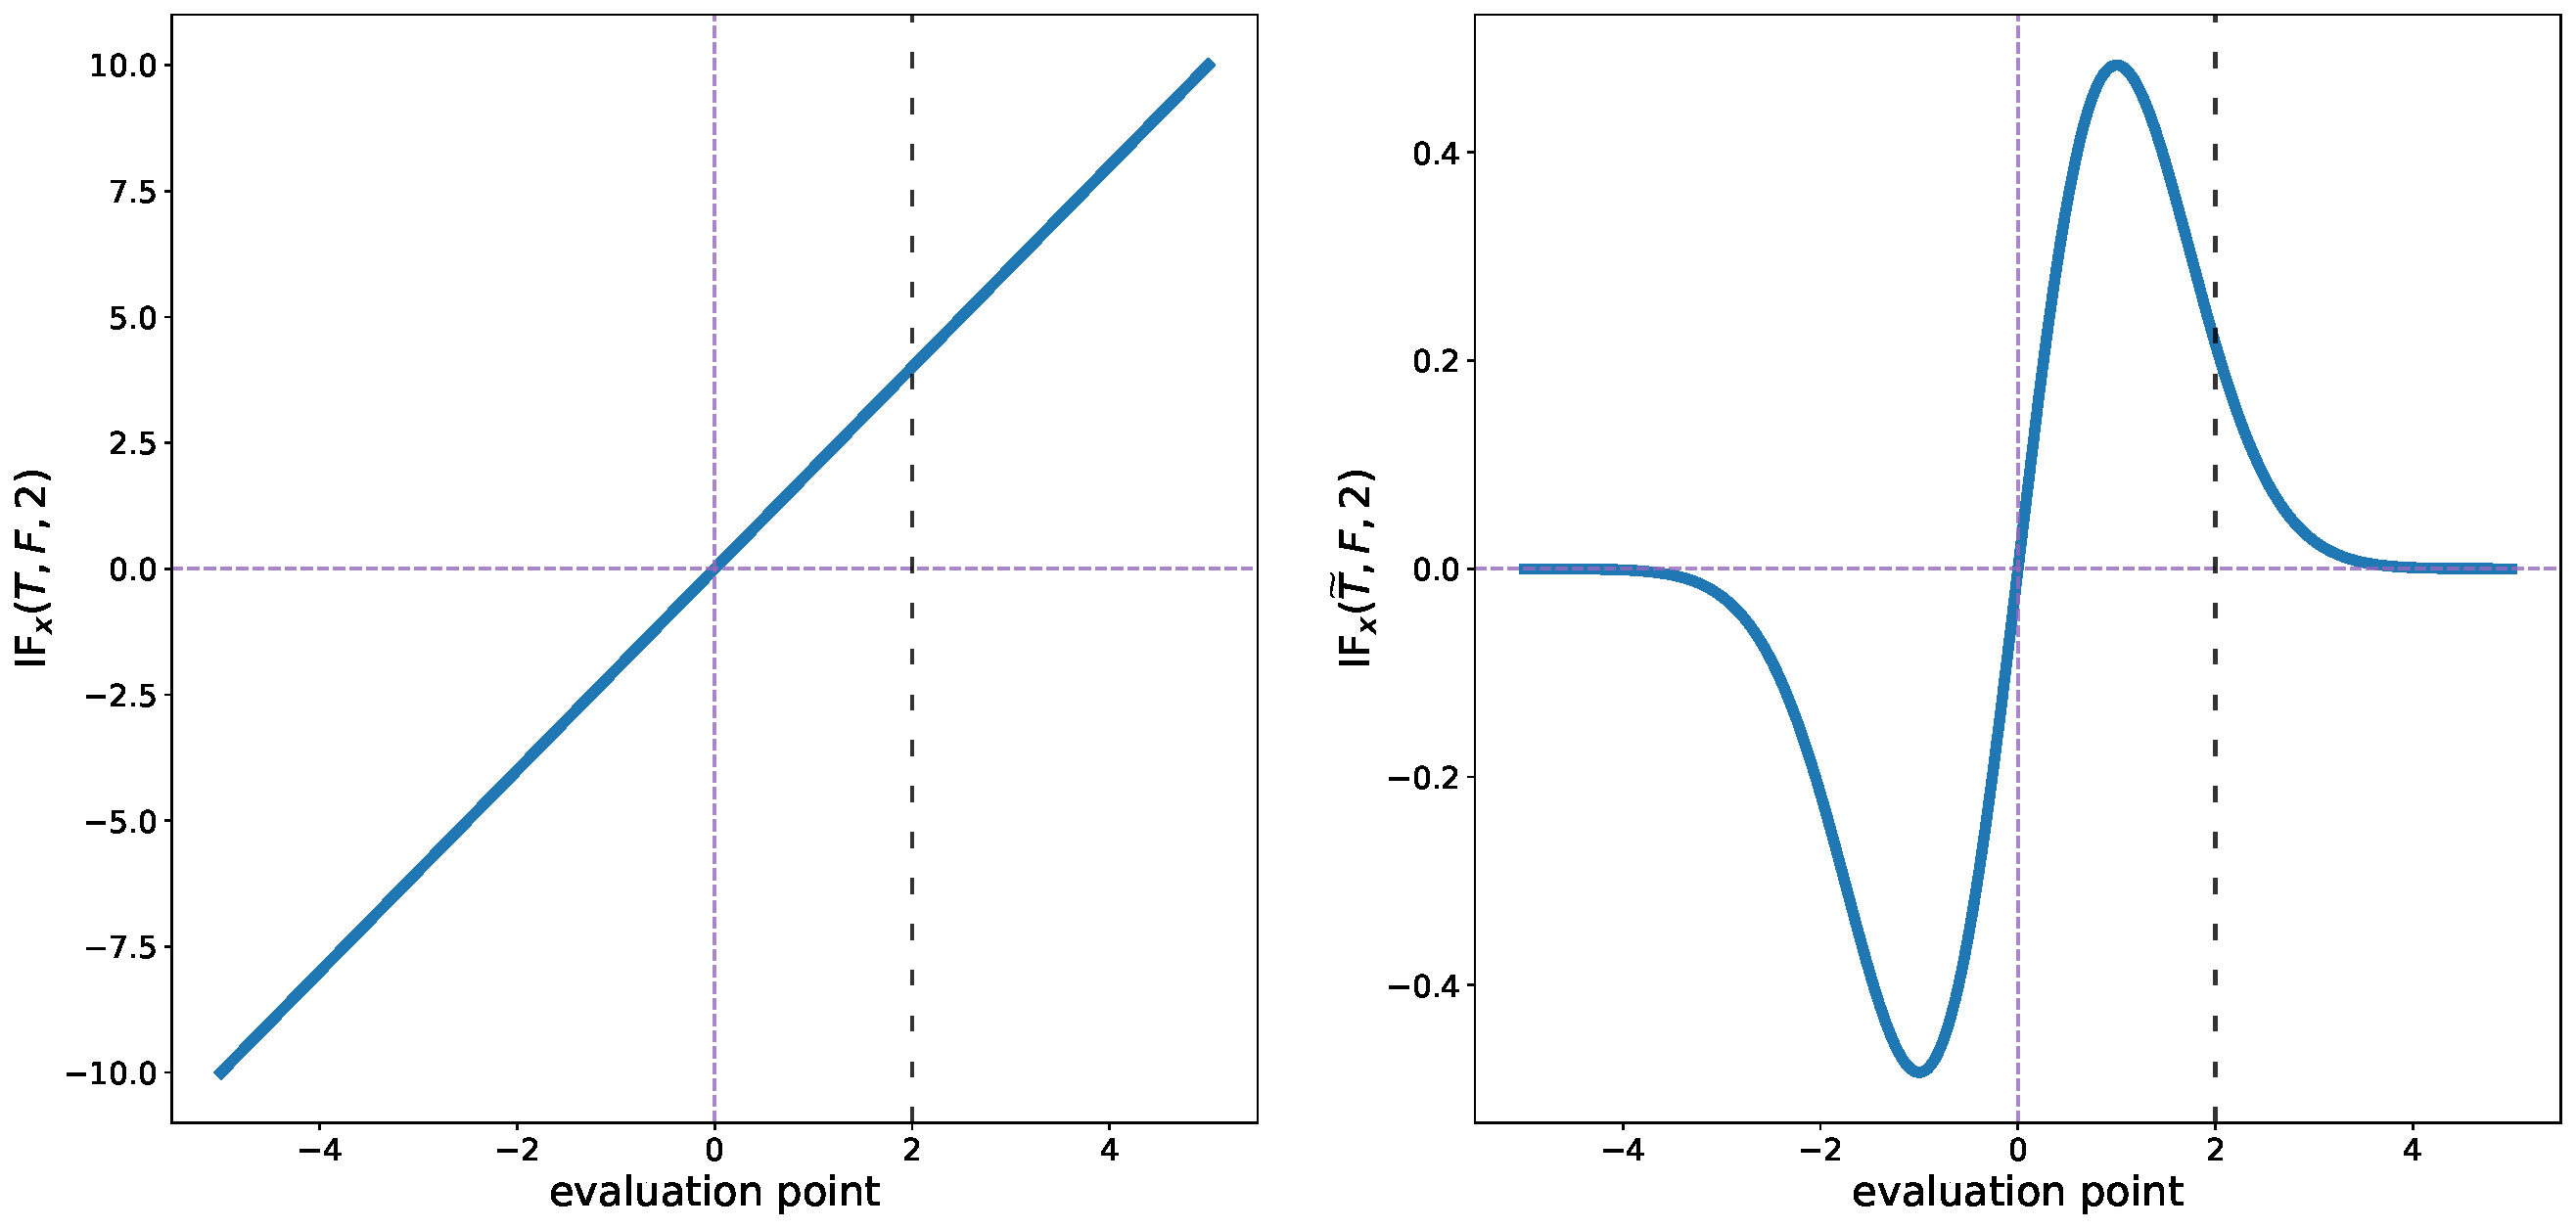
\includegraphics[width=\textwidth]{../plots/comparison-inffunden-inffunlogden-normal-loc-model-mean=0.0-y=2.0.pdf}
	\caption{$\mathrm{IF}_x \parens{T, F, y}$ (left panel) and $\mathrm{IF}_x \parens{\widetilde{T}, F, y}$ (right panel) evaluated at different $x \in \calX$ with $\E_F \bracks{X} = 0$ and $y = 2$. The black dashed vertical line indicates the location of the contaminant $y$. }
	\label{fig-inffun-logden-den-normal-loc-model}
\end{figure}

If we fix $y$ and $F$ and view $\mathrm{IF}_x \parens{T, F, y}$ and $\mathrm{IF}_x \parens{\widetilde{T}, F, y}$ as functions of the evaluation point $x$, both can vary with $x$, which is obvious from Figure \ref{fig-inffun-logden-den-normal-loc-model}. In other words, with a fixed $F$, a fixed $y$ can have different effects on each of $T \parens{F}$ and $\widetilde{T} \parens{F}$ at different evaluation points. In order to have a summarizing quantity to describe the maximal possible effect of $y$ on $T \parens{F}$ and $\widetilde{T} \parens{F}$, we use 
\begin{align*}
	M \parens{T, F, y} := \sup_{x \in \calX} \abs{\mathrm{IF}_x \parens{T, F, y}}, \qquad \text{ and } \qquad
	M \parens{\widetilde{T}, F, y} := \sup_{x \in \calX} \abs{\mathrm{IF}_x \parens{\widetilde{T}, F, y}}, 
\end{align*}
and call them the \textit{overall influences} of $y$ on $T \parens{F}$ and $\widetilde{T} \parens{F}$, respectively. They describe the maximal possible effects of $y$ on $T \parens{F}$ and $\widetilde{T} \parens{F}$, respectively. 

\renewcommand\thmcontinues[1]{continued}
\begin{example}[name=Normal location model, continues=example-normal-loc-model]
	The overall influences of $y$ on $T \parens{F}$ and $\widetilde{T} \parens{F}$ are 
	\begin{align*}
		M \parens{T, F, y} = & \, \begin{cases}
			0, & \, \text{ if } y = \E_F \bracks{X} \\ 
			\infty, & \, \text{ if } y \neq \E_F \bracks{X}
		\end{cases}, \quad \text{ and } \quad 
		M \parens{\widetilde{T}, F, y} = \frac{1}{\sqrt{2 e \pi}} \big\vert y - \E_F \bracks{X} \big\vert, 
	\end{align*}
	respectively. 
	
	Note that, when $y \neq \E_F \bracks{X}$, the overall influence of $y$ on $T \parens{F}$ is infinite, even though the density estimates appear indistinguishable. This infinite overall influence occurs at the two tails by noting $\lim_{x \to \pm \infty} \abs{\mathrm{IF}_x \parens{T, F, y}} = \infty$. This is a potential deficiency of defining the overall influence of $y$ on $T \parens{F}$ to be the supremum norm of $\mathrm{IF}_x \parens{T, F, y}$ taken with respect to the evaluation point $x \in \calX$. 
% the main reason that we have an infinite overall influence is . In other words, this infinite supremum norm occurs at the two tails. This infinite overall influence does \textit{not} imply that log-denisty functions $T \parens{F}$ and $T \parens{\parens{1 - \varepsilon} F + \varepsilon \delta_y}$ are significantly different for an infinitesimal $\varepsilon > 0$, or that denisty functions $\widetilde{T} \parens{F}$ and $\widetilde{T} \parens{\parens{1 - \varepsilon} F + \varepsilon \delta_y}$ are significantly different for an infinitesimal $\varepsilon > 0$. In general, it may \textit{not} be very meaningful to look at an infinite overall influence that occurs at the tails. 
\end{example}

Finally, we define the \textit{sample influence functions of $T \parens{F}$ and $\widetilde{T} \parens{F}$ evaluated at $x \in \calX$} to be 
\begin{align*}
	\mathrm{SIF}_{x, \varepsilon} \parens{T, F, y} := \frac{1}{\varepsilon} \parens[\Big]{T \parens[\big]{\parens{1 - \varepsilon} F + \varepsilon \delta_y} \parens{x} - T \parens{F} \parens{x}}, \\ 
	\mathrm{SIF}_{x, \varepsilon} \parens{\widetilde{T}, F, y} := \frac{1}{\varepsilon} \parens[\Big]{\widetilde{T} \parens[\big]{\parens{1 - \varepsilon} F + \varepsilon \delta_y} \parens{x} - \widetilde{T} \parens{F} \parens{x}}, 
\end{align*}
respectively, and the corresponding \textit{sample overall influences} to be 
\begin{align*}
	\widehat{M}_{\varepsilon} \parens{T, F, y} := \sup_{x \in \calX} \abs{\mathrm{SIF}_{x, \varepsilon} \parens{T, F, y}}, \qquad \text{ and } \qquad
	\widehat{M}_{\varepsilon} \parens{\widetilde{T}, F, y} := \sup_{x \in \calX} \abs{\mathrm{SIF}_{x, \varepsilon} \parens{\widetilde{T}, F, y}}
\end{align*}
respectively. Similarly to \eqref{eq-sample-inffun}, $\mathrm{SIF}_{x, \varepsilon} \parens{T, F, y}$ (\textit{resp.} $\mathrm{SIF}_{x, \varepsilon} \parens{\widetilde{T}, F, y}$) is the finite-difference approximation of $\mathrm{IF}_{x} \parens{T, F, y}$ (\textit{resp.} $\mathrm{IF}_{x, \varepsilon} \parens{\widetilde{T}, F, y}$). 


%The only issue that makes this unusual from the usual definition of an influence function is that you are considering function-valued maps $T$. 
%
%Let $T$ be a map from distributions $F$ on $\calX$ to a function on $\calX$. The influence function is defined to be: $\mathrm{IF} (x; T; F)$
%
%Note that this influence function is itself \textit{function-valued}. We will be using this to study the sensitivity of log-density estimators $T$. So $\mathrm{IF} (x; T; F)$ tells us how the log-density is affected by $x$. 
%
%As I said, the main issue that makes this unusual is that $\mathrm{IF} (x; T; F)$ is function-valued. 
%Overall influence::
%Define $| |$ to be sup norm of functions on $\calX$. Overall influence function: 
%$OIF(x; T; F) = | IF(x; T; F) |$ 


\section{Influence Functions of Density Projections in a Finite-dimensional Exponential Family}\label{section-influence-function-fin-dim-exp-fam}

With the introduction of $\mathrm{IF}_x \parens{T, F, y}$ and $\mathrm{IF}_x \parens{\widetilde{T}, F, y}$ in the preceding section, we focus on the influence functions of the ML and SM density projections (to be defined later) in an $m$-dimensional exponential family $\calQ_{\mathrm{fin}}$ (introduced in Chapter \ref{ch2}) in this section. 

Recall $\calQ_{\mathrm{fin}}$ contains all pdfs of the form 
\begin{align*}
	\tilde{q}_{\theta} \parens{x} := \mu \parens{x} \exp \parens[\big]{\innerp{\theta}{ \varphi \parens{x}} - B \parens{\theta}} \text{ for all } x \in \calX, \qquad \theta \in \Theta, 
\end{align*}
where we assume each component of $\varphi$, $\varphi_j: \calX \to \Real$, is twice continuously differentiable. We define the following maps 
\begin{align*}
	T \parens{F} = & \, \log \tilde{q}_{\theta_{\ML, F}},  && \, \text{ and }  && \, S \parens{F} = \log \tilde{q}_{\theta_{\SM, F}}, \\ 
	\widetilde{T} \parens{F} = & \, \tilde{q}_{\theta_{\ML, F}},  && \, \text{ and } && \, \widetilde{S} \parens{F} = \tilde{q}_{\theta_{\SM, F}}, 
\end{align*}
where $F$ is a distribution function over $\calX$, 
\begin{align*}
	\theta_{\ML, F} := & \, \argmin_{\theta \in \Theta} \braces[\Bigg]{ \int_{\calX} - \log \tilde{q}_{\theta} \parens{x} \mathrm{d} F \parens{x} } \\ 
	= & \, \argmin_{\theta \in \Theta} \braces[\Bigg]{ B \parens{\theta} - \innerp[\Big]{\theta}{ \E_F \bracks{ \varphi \parens{X} } } }, \\ 
	\theta_{\SM, F} := & \, \argmin_{\theta \in \Theta} \braces[\Bigg]{ \int_{\calX} \sum_{u=1}^d \parens[\bigg]{ \frac{1}{2} \parens[\big]{ \partial_u \log \tilde{q}_{\theta} \parens{x}}^2 + \partial_u \log \tilde{q}_{\theta} \parens{x} } \diff F \parens{x} } \\ 
	= & \, \argmin_{\theta \in \Theta} \braces[\Bigg]{ \frac{1}{2} \theta^\top \E_F \bracks{D_1 \parens{X} D_1 \parens{X}^\top } \theta - \theta^\top \E_F \bracks{W \parens{X}}}, 
\end{align*}
$D_1$ is a map from $\calX$ to $\Real^{m \times d}$ with $\bracks{D_1 \parens{x}}_{j, u} = \partial_u \varphi_j \parens{x}$ for all $x \in \calX$, $D_2$ is a map from $\calX$ to $\Real^{m \times d}$ with $\bracks{D_2 \parens{x}}_{j, u} = \partial_u^2 \varphi_j \parens{x}$ for all $x \in \calX$, $W$ is a map from $\calX$ to $\Real^m$ with $W \parens{x} = - \parens{ D_1 \parens{x} \nabla \log \mu \parens{x} + D_2 \parens{x} \boldone_d}$ for all $x \in \calX$, and $\boldone_d := \parens{1, \cdots, 1}^\top \in \Real^d$. Supposing that the pdf of $F$, denoted by $p_0$, exists, we observe that $\widetilde{T} \parens{F}$ and $\widetilde{S} \parens{F}$ are the ML and SM density projections of $p_0$ onto the family $\calQ_{\mathrm{fin}}$, as they have the smallest KL- and H-divergences to $p_0$ among all $\tilde{q}_{\theta} \in \calQ_{\mathrm{fin}}$, respectively. 

Then, the following theorem provides explicit expressions for $\mathrm{IF}_x \parens{T, F, y}$ and $\mathrm{IF}_x \parens{S, F, y}$. The expressions for $\mathrm{IF}_x \parens{\widetilde{T}, F, y}$ and $\mathrm{IF}_x \parens{\widetilde{S}, F, y}$ are easy to obtain by multiplying $\mathrm{IF}_x \parens{T, F, y}$ and $\mathrm{IF}_x \parens{S, F, y}$ with $\widetilde{T} \parens{F} \parens{x}$ and $\widetilde{S} \parens{F} \parens{x}$, respectively, using Proposition \ref{prop-inf-fun-relationship-den-logden}. 

\begin{theorem}[Influence functions of ML and SM log-density projections in $\calQ_{\mathrm{fin}}$ evaluated at $x \in \calX$]\label{theorem-inf-fun-ml-sm-fin-dim-exp-fam}
	\leavevmode
	\begin{enumerate}[label=(\alph*)]
		\item \label{theorem-inf-fun-ml-sm-fin-dim-exp-fam-a} Assume $\E_F \bracks{\varphi \parens{X}}$ exists and belongs to $\interior \parens{\Theta}$, $\int_{\calX} \tilde{q}_{\theta_{\ML, F}} \parens{x} \norm{\varphi \parens{x}}_2^2 \diff x < \infty$, and $\nabla^2 B \parens{\theta_{\ML, F}}$ is invertible. Then, for all $x \in \calX$, 
		\begin{align}\label{eq-inffun-ml-fin-dim-exp-fam}
			\mathrm{IF}_x \parens{T, F, y} = \innerp[\Bigg]{ \widetilde{G}_{\ML} \parens{F, y} }{ \varphi \parens{x} - \int_{\calX} \tilde{q}_{\theta_{\ML, F}} \parens{w} \varphi \parens{w} \diff w }, 
		\end{align}
		where 
		\begin{align*}
			\widetilde{G}_{\ML} \parens{F, y} := \bracks[\big]{\nabla^2 B \parens{\theta_{\ML, F} }}^{-1} \parens[\big]{\varphi \parens{y} - \E_{F} \bracks{\varphi \parens{X}}}
		\end{align*}
		
		\item \label{theorem-inf-fun-ml-sm-fin-dim-exp-fam-b} Assume $\E_F \bracks{W \parens{X}}$ exists, $\int_{\calX} \tilde{q}_{\theta_{\SM, F}} \parens{x} \norm{\varphi \parens{x}}_2^2 \diff x < \infty$, and $\E_F \bracks[\big]{D_1 \parens{X} D_1 \parens{X}^\top}$ is invertible. Then, for all $x \in \calX$, 
		\begin{align}\label{eq-inffun-sm-fin-dim-exp-fam}
			\mathrm{IF}_x \parens{T, F, y} = & \, \innerp[\bigg]{ \widetilde{G}_{\SM} \parens{F, y}}{ \varphi \parens{x} - \int_{\calX} \tilde{q}_{\theta_{\SM, F}} \parens{w} \varphi \parens{w} \diff w}, 
		\end{align}
		where 
		\begin{align*}
			\widetilde{G}_{\SM} \parens{F, y} := & \, \bracks[\Big]{\E_F \bracks[\big]{D_1 \parens{X} D_1 \parens{X}^\top} }^{-1} \times \\ 
			& \qquad \qquad  \braces[\bigg]{W  \parens{y} - D_1 \parens{y} D_1 \parens{y}^\top \bracks[\Big]{\E_F \bracks[\big]{D_1 \parens{X} D_1 \parens{X}^\top} }^{-1} \E_F \bracks{W \parens{X}} }. 
		\end{align*}
	\end{enumerate}
\end{theorem}

The proof of Theorem \ref{theorem-inf-fun-ml-sm-fin-dim-exp-fam} will be provided in Section \ref{proof-theorem-inf-fun-ml-sm-fin-dim-exp-fam}. 

From the proof, we can see $\widetilde{G}_{\ML} \parens{F, y}$ is the influence function of the $M$-estimator $\theta_{\ML, F}$ that satisfies 
\begin{align*}
	0 = \int_{\calX} \parens[\Big]{\nabla B \parens{\theta_{\ML, F}} - \varphi \parens{x}} \diff F \parens{x}, 
\end{align*}
and $\widetilde{G}_{\SM} \parens{F, y}$ is the influence function of the $M$-estimator $\theta_{\SM, F}$ that satisfies 
\begin{align*}
	0 = \E_F \bracks[\big]{D_1 \parens{X} D_1 \parens{X}^\top} \theta_{\SM, F} - \E_F \bracks{W \parens{X}}; 
\end{align*}
in other words, they are the influence functions of their respective natural parameters. % By inspecting the form of \eqref{eq-inffun-ml-fin-dim-exp-fam} and \eqref{eq-inffun-sm-fin-dim-exp-fam}, we see each of them is the inner product between the influence function of the natural parameter and the derivative of the log-density function with respect to $\theta$ evaluated at the unperturbed natural parameter. 

Comparing \eqref{eq-inffun-ml-fin-dim-exp-fam} and \eqref{eq-inffun-sm-fin-dim-exp-fam}, we see that $\mathrm{IF}_x \parens{T, F, y}$ depends on $y$ \emph{only} through the canonical statistics $\varphi$, but $\mathrm{IF}_x \parens{S, F, y}$ depends on $y$ through the first two derivatives of $\varphi$ and the first derivative of $\log \mu$. This is the key difference between $\mathrm{IF}_x \parens{T, F, y}$ and $\mathrm{IF}_x \parens{S, F, y}$. In the examples we will see later, their differences will become more apparent. 

From Theorem \ref{theorem-inf-fun-ml-sm-fin-dim-exp-fam}, we can obtain some properties of $\mathrm{IF}_x \parens{T, F, y}$ and $\mathrm{IF}_x \parens{S, F, y}$ which are given in the corollaries below. 

\begin{corollary}\label{corollary-inffun-fin-dim-exp-fam-zero}
	\leavevmode
	\begin{enumerate}[label=(\alph*)]
		\item \label{corollary-inffun-fin-dim-exp-fam-zero-a} Under the assumptions in Theorem \ref{theorem-inf-fun-ml-sm-fin-dim-exp-fam}\ref{theorem-inf-fun-ml-sm-fin-dim-exp-fam-a}, $\mathrm{IF}_x \parens{T, F, y} = 0$ for all $x \in \calX$ if and only if $F$ and $y$ satisfy 
		\begin{align}\label{eq-corollary-inffun-fin-dim-exp-fam-zero-a}
			\varphi \parens{y} - \E_F \bracks{\varphi \parens{X}} = 0. 
		\end{align} 
		
		\item \label{corollary-inffun-fin-dim-exp-fam-zero-b} Under the assumptions in Theorem \ref{theorem-inf-fun-ml-sm-fin-dim-exp-fam}\ref{theorem-inf-fun-ml-sm-fin-dim-exp-fam-b}, $\mathrm{IF}_x \parens{S, F, y} = 0$ for all $x \in \calX$ if and only if $F$ and $y$ satisfy 
		\begin{align}\label{eq-corollary-inffun-fin-dim-exp-fam-zero-b}
			W \parens{y} - D_1 \parens{y} D_1 \parens{y}^\top \bracks[\Big]{\E_F \bracks[\big]{D_1 \parens{X} D_1 \parens{X}^\top} }^{-1} \E_F \bracks{W \parens{X}} = 0. 
		\end{align}
	\end{enumerate}
\end{corollary}

\begin{corollary}\label{corollary-inffun-fin-dim-exp-fam-bounded}
	\leavevmode
	\begin{enumerate}[label=(\alph*)]
		\item \label{corollary-inffun-fin-dim-exp-fam-bounded-a} Under the assumptions in Theorem \ref{theorem-inf-fun-ml-sm-fin-dim-exp-fam}\ref{theorem-inf-fun-ml-sm-fin-dim-exp-fam-a}, suppose $F$ and $y$ satisfy $\varphi \parens{y} - \E_F \bracks{\varphi \parens{X}} \neq 0$. 
		\begin{enumerate}[label=(\roman*)]
			\item If $\sup_{j = 1, \cdots, m} \ \sup_{x \in \calX} \abs{\varphi_j \parens{x}} < \infty$, then $M \parens{T, F, y} < \infty$. 
			\item If there exists $j^* \in \sets{1, \cdots, m}$ and $x_0 \in \overline{\calX}$ such that $\lim_{x \to x_0} \abs{\varphi_{j^*} \parens{x}} = \infty$ so that $\sup_{x \in \calX} \abs{\varphi_j \parens{x}} = \infty$, $\varphi_{j^*} \parens{y} - \E_F \bracks{\varphi_{j^*} \parens{X}} \neq 0$, and $\lim_{x \to x_0} \frac{\varphi_j \parens{x}}{\varphi_{j^*} \parens{x}} = 0$ for all $j \neq j^*$, then $M \parens{T, F, y} = \infty$. 
		\end{enumerate}
		
		\item \label{corollary-inffun-fin-dim-exp-fam-bounded-b} Under the assumptions in Theorem \ref{theorem-inf-fun-ml-sm-fin-dim-exp-fam}\ref{theorem-inf-fun-ml-sm-fin-dim-exp-fam-b}, suppose $F$ and $y$ satisfy 
		\begin{align*}
			W \parens{y} - D_1 \parens{y} D_1 \parens{y}^\top \bracks[\Big]{\E_F \bracks[\big]{D_1 \parens{X} D_1 \parens{X}^\top} }^{-1} \E_F \bracks{W \parens{X}} \neq 0. 
		\end{align*}
		\begin{enumerate}[label=(\roman*)]
			\item If $\sup_{j = 1, \cdots, m} \ \sup_{x \in \calX} \abs{\varphi_j \parens{x}} < \infty$, then $M \parens{S, F, y} < \infty$. 
			\item If there exists $j^* \in \sets{1, \cdots, m}$ and $x_0 \in \overline{\calX}$ such that $\lim_{x \to x_0} \abs{\varphi_{j^*} \parens{x}} = \infty$ so that $\sup_{x \in \calX} \abs{\varphi_j \parens{x}} = \infty$, the $j^*$-th element of 
			\begin{align*}
				W \parens{y} - D_1 \parens{y} D_1 \parens{y}^\top \bracks[\Big]{\E_F \bracks[\big]{D_1 \parens{X} D_1 \parens{X}^\top} }^{-1} \E_F \bracks{W \parens{X}}
			\end{align*}
			is nonzero, and $\lim_{x \to x_0} \frac{\varphi_j \parens{x}}{\varphi_{j^*} \parens{x}} = 0$ for all $j \neq j^*$, then $M \parens{S, F, y} = \infty$. 
		\end{enumerate}
	\end{enumerate}
\end{corollary}

These corollaries are obvious from Theorem \ref{theorem-inf-fun-ml-sm-fin-dim-exp-fam}, in particular, from \eqref{eq-inffun-ml-fin-dim-exp-fam} and \eqref{eq-inffun-sm-fin-dim-exp-fam}, and their proofs are omitted here. In the rest of this section, we provide several examples to illustrate Theorem \ref{theorem-inf-fun-ml-sm-fin-dim-exp-fam} and Corollaries \ref{corollary-inffun-fin-dim-exp-fam-zero} and \ref{corollary-inffun-fin-dim-exp-fam-bounded}. 

\begin{example}[name=Normal location-scale model]
	Let $\calX = \Real$ and $\calQ$ contain all pdfs of the form 
	\begin{align*}
		\tilde{q}_{\theta} \parens{x} := \frac{1}{\sqrt{2 \pi \sigma^2}} \exp \parens[\bigg]{- \frac{\parens{x - \omega}^2}{2 \sigma^2}} \text{ for all } x \in \mathcal{X}, \qquad \theta := \parens{\omega, \sigma^2} \in \Theta, 
	\end{align*}
	where $\Theta := \mathbb{R} \times \parens{0, \infty}$. In this example, we have 
	\begin{align*}
		\mu \parens{x} = \frac{1}{\sqrt{2 \pi}}, \qquad \varphi \parens{x} = \begin{pmatrix}
			x \\ x^2
		\end{pmatrix}, \qquad B \parens{\theta} = \frac{\omega^2}{2 \sigma^2} + \frac{1}{2} \log \sigma^2, 
	\end{align*}
	and 
	\begin{align*}
		D_1 \parens{x} = \begin{pmatrix}
			1 \\ 2x
		\end{pmatrix}, \qquad D_2 \parens{x} = \begin{pmatrix}
			0 \\ 2
		\end{pmatrix}, \qquad \parens{\log \mu}' \parens{x} = 0, \qquad  W \parens{x} = \begin{pmatrix}
			0 \\ -2
		\end{pmatrix}. 
	\end{align*}
	Assume $m_1 := \E_F \bracks{X}$ and $m_2 := \E_F \bracks{X^2}$ both exist and $m_2 - m_1^2 > 0$. Then, using Theorem \ref{theorem-inf-fun-ml-sm-fin-dim-exp-fam}, we have 
	\begin{align*}
		\mathrm{IF}_x \parens{T, F, y} = & \, \mathrm{IF}_x \parens{S, F, y} = a_1 x^2 + a_2 x + a_3, \qquad \text{ for all } x \in \calX, 
	\end{align*}
	where 
	\begin{align*}
		a_1 := & \, \frac{-m_1}{\parens{m_2 - m_1^2}^2} \parens{y - m_1} + \frac{1}{2 \parens{m_2 - m_1^2}^2} \parens{y^2 - m_2}, \\
		a_2 := & \, \frac{m_2 + m_1^2}{\parens{m_2 - m_1^2}^2} \parens{y - m_1} - \frac{m_1}{\parens{m_2 - m_1^2}^2} \parens{y^2 - m_2}, \\ 
		a_3 := & \, \frac{m_1^3 - 2 m_1 m_2}{\parens{m_2 - m_1^2}^2} \parens{y - m_1} + \frac{m_2}{2 \parens{m_2 - m_1^2}^2} \parens{y^2 - m_2}. 
	\end{align*}
	
	Since, in this example, we have $\varphi_1 \parens{x} = x$ and $\varphi_2 \parens{x} = x^2$ for all $x \in \calX$, and $\sup_{x \in \calX} \vert \varphi_2 \parens{x} \vert = \infty$ with $\lim_{x \to \pm \infty} \varphi_2 \parens{x} = \infty$, and $\lim_{x \to \pm \infty} \frac{\varphi_1 \parens{x}}{\varphi_2 \parens{x}} = 0$, we have $M \parens{T, F, y} = M \parens{S, F, y} = \infty$, which verifies Corollary \ref{corollary-inffun-fin-dim-exp-fam-bounded}. 
	% If $m_1 \neq y$ or $m_2 \neq y^2$, we have 
%	and 
%	\begin{align*}
%		\mathrm{IF}_x \parens{\widetilde{T}, F, y} = & \, \mathrm{IF}_x \parens{\widetilde{S}, F, y} = \tilde{q}_{\parens{m_1, m_2 - m_1^2}} \parens{x} \parens{a_1 x^2 + a_2 x + a_3}, \qquad \text{ for all } x \in \calX, \\ 
%		M \parens{\widetilde{T}, F, y} = & \, M \parens{\widetilde{S}, F, y} =  , 
%	\end{align*}
\end{example}


\begin{example}[name=Lognormal location model]
	Let $\mathcal{X} = \parens{0, \infty}$ and $\calQ$ contain all pdfs of the form 
	\begin{align*}
		\tilde{q}_{\theta} \parens{x} := \frac{1}{x \sqrt{2 \pi}} \exp \parens[\bigg]{- \frac{\parens{\log x - \theta}^2}{2}} \text{ for all } x \in \calX, \qquad \theta \in \Real. 
	\end{align*}
	In this example, we have 
	\begin{align*}
		\mu \parens{x} = \frac{1}{x \sqrt{2 \pi}} \exp \parens[\bigg]{- \frac{\parens{\log x}^2}{2}}, \qquad \varphi \parens{x} = \log x, \qquad B \parens{\theta} = \frac{\theta^2}{2}, 
	\end{align*}
	and 
	\begin{align*}
		D_1 \parens{x} = \frac{1}{x}, \quad D_2 \parens{x} = - \frac{1}{x^2}, \quad \parens{\log \mu}' \parens{x} = -\frac{1}{x} - \frac{\log x}{x}, \quad W \parens{x} = \frac{2}{x^2} + \frac{\log x}{x^2}. 
	\end{align*}
	Then, using Theorem \ref{theorem-inf-fun-ml-sm-fin-dim-exp-fam}, we obtain 
	\begin{align*}
		\mathrm{IF}_x \parens{T, F, y} = & \, \parens[\big]{\log y - m_1 } \parens[\big]{\log x - m_1 }, \\ 
		\mathrm{IF}_x \parens{S, F, y} = & \, \frac{1}{m_3 y^2} \parens[\bigg]{\log y - \frac{m_2}{m_3}} \parens[\bigg]{\log x - 2 - \frac{m_2}{m_3}}, 
	\end{align*}
	for all $x \in \calX$, where we assume $m_1 := \E_F \bracks{\log X}$, $m_2 := \E_F \bracks{X^{-2} \log X}$ and $m_3 := \E_F \bracks{X^{-2}}$ exist. 
	
	In particular, $\mathrm{IF}_x \parens{T, F, y} = 0$ for all $x \in \calX$ if and only if $F$ and $y$ satisfy $\log y = m_1$, which is exactly \eqref{eq-corollary-inffun-fin-dim-exp-fam-zero-a}; and, $\mathrm{IF}_x \parens{S, F, y} = 0$ for all $x \in \calX$ if and only if $F$ and $y$ satisfy $\log y - \frac{m_2}{m_3} = 0$, which is exactly \eqref{eq-corollary-inffun-fin-dim-exp-fam-zero-b}. These illustrate Corollary \ref{corollary-inffun-fin-dim-exp-fam-zero}. 
	
	Also, note that, in this example, $\sup_{x \in \calX} \abs{\varphi \parens{x}} = \sup_{x \in \calX} \abs{\log x} = \infty$. Supposing $\log y - \E_F \bracks{\log X} \neq 0$, we have $M \parens{T, F, y} = \infty$, which illustrates Corollary \ref{corollary-inffun-fin-dim-exp-fam-bounded}\ref{corollary-inffun-fin-dim-exp-fam-bounded-a}; supposing $\log y - \frac{m_2}{m_3} \neq 0$, we have $M \parens{S, F, y} = \infty$, which illustrates Corollary \ref{corollary-inffun-fin-dim-exp-fam-bounded}\ref{corollary-inffun-fin-dim-exp-fam-bounded-b}. 
%	For fixed $x \in \calX$ and $F$, the larger the value of $y$ is, the larger the value of $\mathrm{IF}_x \parens{T, F, y}$ is. 
%	For fixed $x \in \calX$ and $F$, 
%	\begin{itemize}
%		\item if $y \in \parens[\Big]{0, \exp \parens[\big]{\frac{m_1}{m_2} + \frac{1}{2}}}$, the larger $y$ is, the larger $\mathrm{IF}_x \parens{S, F, y}$ is; 
%		\item if $y > \exp \parens[\big]{\frac{m_1}{m_2} + \frac{1}{2}}$, the larger $y$ is, the smaller $\mathrm{IF}_x \parens{S, F, y}$ is. 
%	\end{itemize}
\end{example}


\begin{example}[name=Gamma rate model]
	Let $\calX = \parens{0, \infty}$ and $\calQ$ contain all pdfs of the form 
	\begin{align*}
		\tilde{q}_{\theta} \parens{x} := \frac{x^{\alpha-1}}{\Gamma \parens{\alpha}} \exp \parens[\Big]{- \theta x + \alpha \log \theta} \text{ for all } x \in \calX, \qquad \theta \in \parens{0, \infty}. 
	\end{align*}
	We assume $\alpha > 1$ is known. In this example 
	\begin{align*}
		\mu \parens{x} = \frac{x^{\alpha-1}}{\Gamma \parens{\alpha}}, \qquad \varphi \parens{x} = - x, \qquad B \parens{\theta} = - \alpha \log \theta, 
	\end{align*}
	and 
	\begin{align*}
		D_1 \parens{x} = -1, \quad D_2 \parens{x} = 0, \quad \parens{\log \mu}' \parens{x} = \frac{\alpha - 1}{x}, \quad W \parens{x} = \frac{\alpha - 1}{x}. 
	\end{align*}
	Then, using Theorem \ref{theorem-inf-fun-ml-sm-fin-dim-exp-fam}, we obtain 
	\begin{align*}
		\mathrm{IF}_x \parens{T, F, y} = & \, \frac{\alpha}{m_1^2} \parens{y - m_1} \parens{x - m_1}, \\ 
		\mathrm{IF}_x \parens{S, F, y} = & \, \parens{\alpha - 1} \parens{m_2 - y^{-1} } \parens[\bigg]{x - \frac{\alpha}{\alpha - 1} \frac{1}{m_2}}, 
	\end{align*}
	for all $x \in \calX$, where we assume $m_1 := \E_F \bracks{X}$ and $m_2 := \E_F \bracks{X^{-1}}$ exist. 
	
	In particular, $\mathrm{IF}_x \parens{T, F, y} = 0$ for all $x \in \calX$ if and only if $F$ and $y$ satisfy $y = m_1$, which is exactly \eqref{eq-corollary-inffun-fin-dim-exp-fam-zero-a}; and, $\mathrm{IF}_x \parens{S, F, y} = 0$ for all $x \in \calX$ if and only if $F$ and $y$ satisfy $y^{-1} - m_2 = 0$, which is exactly \eqref{eq-corollary-inffun-fin-dim-exp-fam-zero-b}. These illustrate Corollary \ref{corollary-inffun-fin-dim-exp-fam-zero}. 
	
	Note that, in this example, $\sup_{x \in \calX} \abs{\varphi \parens{x}} = \sup_{x \in \calX} \abs{-x} = \infty$. Supposing $\E_F \bracks{X} - y \neq 0$, we have $M \parens{T, F, y} = \infty$, which illustrates Corollary \ref{corollary-inffun-fin-dim-exp-fam-bounded}\ref{corollary-inffun-fin-dim-exp-fam-bounded-a}; supposing $m_2 - y^{-1} \neq 0$, we have $M \parens{S, F, y} = \infty$, which illustrates Corollary \ref{corollary-inffun-fin-dim-exp-fam-bounded}\ref{corollary-inffun-fin-dim-exp-fam-bounded-b}. 
%	For fixed $x \in \calX$ and $F$, the larger the value of $y$ is, the larger the value of $\mathrm{IF}_x \parens{T, F, y}$ is. 
%	For fixed $x \in \calX$ and $F$, the larger the value of $y$ is, the larger the value of $\mathrm{IF}_x \parens{S, F, y}$ is. 
\end{example}

\section{Influence Functions of Density Projections in a Kernel Exponential Family}\label{section-influence-function-kernel-exp-fam}

We now turn to the influence functions of the ML and SM density projections in a kernel exponential family $\calQ_{\ker}$ (introduced in Chapter \ref{ch2}) in this section. Recall $\calQ_{\ker}$ contains all pdfs of the form 
\begin{align*}
	q_{f} \parens{x} := \mu \parens{x} \exp \parens[\big]{f \parens{x} - A \parens{f}} \text{ for all } x \in \calX, \qquad f \in \calF \subseteq \calH. 
\end{align*}

We still let $F$ be a distribution function over $\calX$, and define the following maps 
\begin{align*}
	T_{\lambda} \parens{F} = & \, \log q_{f_{\ML, F}^{\parens{\lambda}}},  && \, \text{ and }  && \, S_{\rho} \parens{F} = \log q_{f_{\SM, F}^{\parens{\rho}}}, \\ 
	\widetilde{T}_{\lambda} \parens{F} = & \, q_{f_{\ML, F}^{\parens{\lambda}}},  && \, \text{ and }  && \, \widetilde{S}_{\rho} \parens{F} = q_{f_{\SM, F}^{\parens{\rho}}}, 
\end{align*}
where 
\begin{align}
	f_{\ML, F}^{\parens{\lambda}} := & \, \argmin_{f \in \calF} \braces[\Bigg]{A \parens{f} - \int_{\calX} f \parens{x} \diff F \parens{x} + \frac{\lambda}{2} \norm{f}_{\calH}^2}, \label{eq-ml-obj-fun-general} \\ 
	f_{\SM, F}^{\parens{\rho}} := & \, \argmin_{f \in \calF} \braces[\Bigg]{\frac{1}{2} \innerp{f}{C_{F} f}_{\calH} - \innerp{f}{z_{F}}_{\calH} + \frac{\rho}{2} \norm{f}_{\calH}^2}, \label{eq-sm-obj-fun-general}
\end{align}
with $C_F := \int_{\calX} \sum_{u=1}^d \partial_u k \parens{x, \,\cdot\,} \otimes \partial_u k \parens{x, \,\cdot\,} \diff F \parens{x}$ mapping from $\calH$ to $\calH$, and $z_F := - \int_{\calX} \sum_{u=1}^d \parens{\partial_u \log \mu \parens{x} \partial_u k \parens{x, \,\cdot\,} + \partial_u^2 k \parens{x, \,\cdot\,}} \diff F \parens{x} \in \calH$. If the distribution function $F$ has a pdf $p_0$, the resulting $C_F$ is \eqref{eq-C-def} defined in Chapter \ref{ch3}; if $F = F_n$, the empirical distribution function of data $X_1, \cdots, X_n$, the resulting $C_{F_n}$ is $\widehat{C}$ defined in \eqref{eq-hatC} in Chapter \ref{ch2}. 

Note that both objective functionals in \eqref{eq-ml-obj-fun-general} and \eqref{eq-sm-obj-fun-general} are strongly convex with constants $\lambda > 0$ and $\rho > 0$, respectively. It follows that each of $f_{\ML, F}^{\parens{\lambda}}$ and $f_{\SM, F}^{\parens{\rho}}$ exists and is unique  \parencite[Corollary 11.17 in][]{Bauschke2017-he}. 

We then have the following results on the influence functions of the penalized ML and SM log-density projections onto $\calQ_{\ker}$ evaluated at $x \in \calX$. 

\begin{theorem}[Influence functions of ML and SM log-density projections in $\calQ_{\ker}$ evaluated at $x \in \calX$]\label{theorem-inf-fun-ml-sm-ker-exp-fam}
\leavevmode
	\begin{enumerate}[label=(\alph*)]
		\item \label{theorem-inf-fun-ml-sm-ker-exp-fam-a} Under \ref{assumption-2-1-inf-dim} - \ref{assumption-2-4-base-density} in Chapter \ref{ch2}, we have, for all $x \in \calX$, 
		\begin{align}\label{eq-inf-fun-ml-ker-exp-fam}
			\mathrm{IF}_x \parens{T_{\lambda}, F, y} = & \, \innerp[\Bigg]{G_{\ML} \parens{F, y}}{ k \parens{x, \,\cdot\,} - \int_{\calX} k \parens{w, \,\cdot\,} q_{f_{\ML, F}^{\parens{\lambda}}} \parens{w} \diff w }_{\calH}, 
		\end{align}
		where
		\begin{align*}
			G_{\ML} \parens{F, y} := & \, \Bigg\{\E_{q_{f_{\ML, F}^{\parens{\lambda}}}} \bracks[\Big]{ \parens[\big]{k \parens{X, \,\cdot\,} - \Upsilon } \otimes \parens[\big]{k \parens{X, \,\cdot\,} - \Upsilon }} + \lambda I \Bigg\}^{-1} \bigg( k \parens{y, \,\cdot\,} -  \\ 
			& \qquad \int_{\calX} k \parens{x, \,\cdot\,} \diff F \parens{x} \bigg) \in \calH, 
		\end{align*}
		and $\Upsilon := \int_{\calX} k \parens{x, \,\cdot\,} q_{f_{\ML, F}^{\parens{\lambda}}}\parens{x} \diff x \in \calH$. 
		
		\item \label{theorem-inf-fun-ml-sm-ker-exp-fam-b} Under \ref{assumption-2-1-inf-dim} - \ref{assumption-2-4-base-density} in Chapter \ref{ch2} and \ref{assumption-1} - \ref{assumption-5} in Chapter \ref{ch3}, we have, for all $x \in \calX$, 
		\begin{align}
			\mathrm{IF}_x \parens{S_{\rho}, F, y} = & \, \innerp[\Bigg]{G_{\SM} \parens{F, y}}{k \parens{x, \,\cdot\,} - \int_{\calX} k \parens{w, \,\cdot\,} q_{f_{\SM, F}^{\parens{\rho}}} \parens{w} \diff w}_{\calH}, 
		\end{align}
		where 
		\begin{align*}
			G_{\SM} \parens{F, y} := & \, \parens{C_{F} + \rho I}^{-1} \parens[\Big]{z_{\delta_y} - \parens{C_{\delta_y} + \rho I} \parens{C_{F} + \rho I}^{-1} z_{F}} \in \calH. 
		\end{align*}
	\end{enumerate}
\end{theorem}

The proof of Theorem \ref{theorem-inf-fun-ml-sm-ker-exp-fam} can be found in Section \ref{proof-theorem-inf-fun-ml-sm-ker-exp-fam}. 	

Comparing Theorems \ref{theorem-inf-fun-ml-sm-fin-dim-exp-fam} and \ref{theorem-inf-fun-ml-sm-ker-exp-fam}, we see they share many similarities. In particular, $\mathrm{IF}_x \parens{T_{\lambda}, F, y}$ depends on $y$ through $k$ \emph{only}, but $\mathrm{IF}_x \parens{S_{\rho}, F, y}$ depends on $y$ through the first two partial derivatives of $k$ and the first derivative of $\log \mu$. Moreover, $G_{\ML} \parens{F, y}$ is the influence function of the $M$-estimator $f_{\ML, F}^{\parens{\lambda}}$ that satisfies 
\begin{align*}
	0 = \int_{\calX} \parens[\Big]{\nabla A \parens{f_{\ML, F}^{\parens{\lambda}}} - k \parens{x, \,\cdot\,} + \lambda f_{\ML, F}^{\parens{\lambda}}} \diff F \parens{x}, 
\end{align*}
and $G_{\SM} \parens{F, y}$ is the influence function of the $M$-estimator $f_{\SM, F}^{\parens{\rho}}$ that satisfies 
\begin{align*}
	0 = C_F f_{\SM, F}^{\parens{\rho}} - z_{F} + \rho f_{\ML, F}^{\parens{\rho}}. 
\end{align*}
The covariance operator 
\begin{align*}
	\E_{q_{f_{\ML, F}^{\parens{\lambda}}}} \bracks[\Big]{ \parens[\big]{k \parens{X, \,\cdot\,} - \Upsilon } \otimes \parens[\big]{k \parens{X, \,\cdot\,} - \Upsilon }}
\end{align*}
appearing in $G_{\ML} \parens{F, y}$ plays the role of $\nabla^2 B \parens{\theta_{\ML, F} }$ in $\widetilde{G}_{\ML} \parens{F, y}$, where $\nabla^2 B \parens{\theta_{\ML, F} }$ is the covariance matrix of $\varphi$ under $\tilde{q}_{\theta_{\ML, F}}$. The operator $C_F$ appearing in $G_{\SM} \parens{F, y}$ plays the role of $\E_F \bracks{D_1 \parens{X} D_1 \parens{X}^{\top}}$ in $\widetilde{G}_{\SM} \parens{F, y}$, and $z_F$ in $G_{\SM} \parens{F, y}$ plays the role of $\E_F \bracks{W \parens{X}}$ in $\widetilde{G}_{\SM} \parens{F, y}$. 

Even though Theorem \ref{theorem-inf-fun-ml-sm-ker-exp-fam} provides explicit expressions of $\mathrm{IF}_x \parens{T_{\lambda}, F, y}$ and $\mathrm{IF}_x \parens{S_{\rho}, F, y}$, they are hard to work with directly to compare the sensitivities of the penalized ML and SM density estimators. We will work with the sample influence function in the next chapter and compare their sensitivities numerically. 

\newpage

\section{Proofs}

\subsection{Proof of Proposition \ref{prop-inf-fun-relationship-den-logden}}\label{proof-prop-inf-fun-relationship-den-logden}

\begin{proof}[Proof of Proposition \ref{prop-inf-fun-relationship-den-logden}]
	Under the assumption in the proposition and with an application of the chain rule, we have 
	\begin{align*}
		\mathrm{IF}_x \parens{\widetilde{T}, F, y} = & \, \frac{\diff}{\diff \varepsilon} \parens[\Big]{\widetilde{T} \parens[\big]{\parens{1 - \varepsilon} F + \varepsilon \delta_y} \parens{x} } \bigg\vert_{\varepsilon = 0} \\ 
		= & \, \frac{\diff}{\diff \varepsilon} \parens[\Big]{\exp \parens[\big]{T \parens{\parens{1 - \varepsilon} F + \varepsilon \delta_y} \parens{x} }} \bigg\vert_{\varepsilon = 0} \\ 
		= & \, \exp \parens[\big]{T \parens{F} \parens{x} } \frac{\diff}{\diff \varepsilon} \parens[\Big]{T \parens[\big]{\parens{1 - \varepsilon} F + \varepsilon \delta_y} \parens{x} } \bigg\vert_{\varepsilon = 0} \\ 
		= & \, \widetilde{T} \parens{F} \parens{x} \mathrm{IF}_x \parens{T, F, y}. 
	\end{align*}
\end{proof}


\subsection{Proof of Proposition \ref{prop-inf-fun-relationship-den-logden-kldiv}}\label{proof-prop-inf-fun-relationship-den-logden-kldiv}

\begin{proof}[Proof of Proposition \ref{prop-inf-fun-relationship-den-logden-kldiv}]
	Let $\varepsilon \in \parens{0, 1}$. By the definition of the KL-divergence, we have 
	\begin{align*}
		\mathrm{KL} \parens[\Big]{\widetilde{T} \parens{F} \big\Vert \widetilde{T} \parens{\parens{1 - \varepsilon} F + \varepsilon \delta_y}} = - \int_{\calX} \widetilde{T} \parens{F} \parens{x} \parens[\Big]{T \parens{ \parens{1 - \varepsilon} F + \varepsilon \delta_y} \parens{x} - T \parens{F} \parens{x} } \diff x. 
	\end{align*}
	Differentiating both sides wrt $\varepsilon$, interchanging differentiation and integral (which is allowed by the assumptions), and evaluating at $\varepsilon = 0$, we have 
	\begin{align*}
		& \, \frac{\diff}{\diff \varepsilon} \mathrm{KL} \parens[\Big]{\widetilde{T} \parens{F} \big\Vert \widetilde{T} \parens{\parens{1 - \varepsilon} F + \varepsilon \delta_y}} \bigg\vert_{\varepsilon=0} \\ 
		= & \, - \int_{\calX} \widetilde{T} \parens{F} \parens{x} \frac{\diff}{\diff \varepsilon} \parens[\Big]{T \parens{ \parens{1 - \varepsilon} F + \varepsilon \delta_y} \parens{x} - T \parens{F} \parens{x}} \bigg\vert_{\varepsilon=0} \diff x \\ 
		= & \, - \int_{\calX} \widetilde{T} \parens{F} \parens{x} \mathrm{IF}_x \parens{T, F, y} \diff x \\ 
		= & \, - \int_{\calX} \mathrm{IF}_x \parens{\widetilde{T}, F, y} \diff x, 
	\end{align*}
	where the last equality follows from Proposition \ref{prop-inf-fun-relationship-den-logden}. 
\end{proof}


\subsection{Proof of Theorem \ref{theorem-inf-fun-ml-sm-fin-dim-exp-fam}} \label{proof-theorem-inf-fun-ml-sm-fin-dim-exp-fam}

\begin{proof}[Proof of Theorem \ref{theorem-inf-fun-ml-sm-fin-dim-exp-fam}]
	For simplicity, we let $F_{\varepsilon} := \parens{1 - \varepsilon} F + \varepsilon \delta_y$ for $\varepsilon \in \parens{0, 1}$. 
	
	\ref{theorem-inf-fun-ml-sm-fin-dim-exp-fam-a} First note 
	\begin{align*}
		\frac{1}{\varepsilon} \parens[\Big]{T \parens{ F_{\varepsilon}} \parens{x} - T \parens{F} \parens{x}} 
		= \innerp[\bigg]{\frac{1}{\varepsilon} \parens[\big]{\theta_{\ML, F_{\varepsilon}} - \theta_{\ML, F}} }{ \varphi \parens{x}} - \frac{1}{\varepsilon} \parens[\Big]{B \parens{\theta_{\ML, F_{\varepsilon}}} - B \parens{\theta_{\ML, F}}}. 
	\end{align*}
	If we let $\varepsilon \to 0^+$ on both sides and use the chain rule, we have 
	\begin{align*}
		& \, \lim_{\varepsilon \to 0^+} \frac{1}{\varepsilon} \parens[\Big]{T \parens{ F_{\varepsilon}} \parens{x} - T \parens{F} \parens{x}} \\ 
		% = & \, \innerp[\bigg]{ \frac{1}{\varepsilon} \parens[\Big]{\theta_1 \parens[\big]{\parens{1 - \varepsilon} F + \varepsilon \delta_y} - \theta_1 \parens{F}}}{ \varphi \parens{x}} - \lim_{\varepsilon \to 0^+} \frac{1}{\varepsilon} \parens[\Big]{B \parens[\big]{\theta_1 \parens{\parens{1 - \varepsilon} F + \varepsilon \delta_y}} - B \parens{\theta_1 \parens{F}}} \nonumber \\ 
		= & \, \innerp[\bigg]{ \lim_{\varepsilon \to 0^+} \frac{1}{\varepsilon} \parens[\big]{\theta_{\ML, F_{\varepsilon}} - \theta_{\ML, F} } }{ \varphi \parens{x}} - \int_{\calX} \tilde{q}_{\theta_{\ML, F}} \parens{w} \innerp[\Bigg]{ \lim_{\varepsilon \to 0^+} \frac{1}{\varepsilon} \parens[\big]{\theta_{\ML, F_{\varepsilon}} - \theta_{\ML, F} } }{ \varphi \parens{w} } \diff w, 
	\end{align*}
	which exists if the limit $\lim_{\varepsilon \to 0^+} \frac{1}{\varepsilon} \parens{\theta_{\ML, F_{\varepsilon}} - \theta_{\ML, F} }$ exists. The desired result follows if we can show 
	\begin{align}\label{eq-inffun-ml-nat-param-fin-dim-exp-fam}
		\lim_{\varepsilon \to 0^+} \frac{1}{\varepsilon} \parens[\big]{ \theta_{\ML, F_{\varepsilon}} - \theta_{\ML, F}} = \bracks[\big]{\nabla^2 B \parens{\theta_{\ML, F}}}^{-1} \parens[\big]{\varphi \parens{y} - \E_{F} \bracks{\varphi \parens{X}}}. 
	\end{align}
	
	Note the LHS of \eqref{eq-inffun-ml-nat-param-fin-dim-exp-fam} is the influence function of the $M$-estimator defined by 
	\begin{align*}
		0 = \int_{\calX} \parens[\Big]{\nabla B \parens{\theta_{\ML, F}} - \varphi \parens{x}} \diff F \parens{x}. 
	\end{align*}
	Using the result in Example \ref{example-inf-fun-m-estimator}, we can see \eqref{eq-inffun-ml-nat-param-fin-dim-exp-fam} follows, which completes the proof. 
	
%	Notice that $\theta_1 \parens{\parens{1 - \varepsilon} F + \varepsilon \delta_y}$ is an $M$-estimator and must satisfy 
%	\begin{align*}
%		0 = & \, \int_{\calX} \parens[\Big]{\nabla B \parens[\big]{\theta_1 \parens{ \parens{1 - \varepsilon} F + \varepsilon \delta_y}} - \varphi \parens{x}} \diff \parens[\big]{ \parens{1 - \varepsilon} F + \varepsilon \delta_y} \parens{x} \nonumber \\ 
%		= & \, \nabla B \parens[\big]{\theta_1 \parens{ \parens{1 - \varepsilon} F + \varepsilon \delta_y}} - \int_{\calX} \varphi \parens{x} \diff \parens[\big]{ \parens{1 - \varepsilon} F + \varepsilon \delta_y} \parens{x}. 
%	\end{align*}
%	Differentiating both sides of the preceding equation with respect to $\varepsilon$ yields 
%	\begin{align*}
%		0 = & \, \nabla^2 B \parens[\big]{\theta_1 \parens{\parens{1 - \varepsilon} F + \varepsilon \delta_y}} \frac{\diff}{\diff \varepsilon} \theta_1 \parens{\parens{1 - \varepsilon} F + \varepsilon \delta_y} - \int_{\calX} \varphi \parens{x} \diff \parens[\big]{ - F + \delta_y} \parens{x}. 
%	\end{align*}
%	Letting $\varepsilon \to 0^+$ on both sides, we obtain 
%	\begin{align*}
%		0 = & \, \nabla^2 B \parens[\big]{\theta_1 \parens{F}} \bracks[\Bigg]{\frac{\diff}{\diff \varepsilon} \theta_1 \parens{\parens{1 - \varepsilon} F + \varepsilon \delta_y}\bigg\vert_{\varepsilon = 0}} + \E_{F} \bracks{\varphi \parens{x}} - \varphi \parens{y}. 
%	\end{align*}
%	Rearranging terms in the preceding equation, we have 
%	\begin{align*}
%		\lim_{\varepsilon \to 0^+} \frac{1}{\varepsilon} \parens[\Big]{ \theta_1 \parens[\big]{\parens{1 - \varepsilon} F + \varepsilon \delta_y} - \theta_1 \parens{F}} = & \, \frac{\diff}{\diff \varepsilon} \theta_1 \parens{\parens{1 - \varepsilon} F + \varepsilon \delta_y} \bigg\vert_{\varepsilon = 0} \nonumber \\ 
%		= & \, \bracks[\big]{\nabla^2 B \parens{\theta_1 \parens{F}}}^{-1} \parens[\big]{\varphi \parens{y} - \E_{F} \bracks{\varphi \parens{X}}}. 
%	\end{align*}
	
	\ref{theorem-inf-fun-ml-sm-fin-dim-exp-fam-b}  Similar to \ref{theorem-inf-fun-ml-sm-fin-dim-exp-fam-a}, we have 
	\begin{align*}
		& \, \lim_{\varepsilon \to 0^+} \frac{1}{\varepsilon} \parens[\Big]{S \parens{ F_{\varepsilon}} \parens{x} - S \parens{F} \parens{x}} \\ 
		= & \, \innerp[\bigg]{ \lim_{\varepsilon \to 0^+} \frac{1}{\varepsilon} \parens[\big]{\theta_{\SM, F_{\varepsilon}} - \theta_{\SM, F} } }{ \varphi \parens{x}} - \int_{\calX} \tilde{q}_{\theta_{\SM, F}} \parens{w} \innerp[\Bigg]{ \lim_{\varepsilon \to 0^+} \frac{1}{\varepsilon} \parens[\big]{\theta_{\SM, F_{\varepsilon}} - \theta_{\SM, F} } }{ \varphi \parens{w} } \diff w, 
	\end{align*}
	which exists if the limit $\lim_{\varepsilon \to 0^+} \frac{1}{\varepsilon} \parens{\theta_{\SM, F_{\varepsilon}} - \theta_{\SM, F} }$ exists. The desired result follows if we can show 
	\begin{align}
		& \, \lim_{\varepsilon \to 0^+} \parens[\big]{\theta_{\SM, F_{\varepsilon}} - \theta_{\SM, F}} = \bracks[\Big]{\E_F \bracks[\big]{D_1 \parens{X} D_1 \parens{X}^\top} }^{-1} \times \nonumber \\ 
		& \qquad \qquad \braces[\bigg]{W \parens{y} - D_1 \parens{y} D_1 \parens{y}^\top \bracks[\Big]{\E_F \bracks[\big]{D_1 \parens{X} D_1 \parens{X}^\top} }^{-1} \E_F \bracks{W \parens{X}} }. \label{eq-inffun-sm-nat-param-fin-dim-exp-fam}
	\end{align}
	
	Note the LHS of \eqref{eq-inffun-sm-nat-param-fin-dim-exp-fam} is the influence function of the $M$-estimator defined by 
	\begin{align*}
		0 = \E_F \bracks[\big]{D_1 \parens{X} D_1 \parens{X}^\top} \theta_{\SM, F} - \E_F \bracks{W \parens{X}}. 
	\end{align*}
	Using the result in Example \ref{example-inf-fun-m-estimator}, we can see \eqref{eq-inffun-sm-nat-param-fin-dim-exp-fam} follows, which completes the proof. 
	
%	What remains to show is 
%	\begin{align*}
%		& \, \lim_{\varepsilon \to 0^+} \frac{1}{\varepsilon} \parens[\Big]{\theta_2 \parens[\big]{\parens{1 - \varepsilon} F + \varepsilon \delta_y} - \theta_2 \parens{F}} \\ 
%		= & \, \bracks[\Big]{\E_F \bracks[\big]{D_1 \parens{X} D_1 \parens{X}^\top} }^{-1} \bigg\{S \parens{y} - D_1 \parens{y} D_1 \parens{y}^\top \bracks[\Big]{\E_F \bracks[\big]{D_1 \parens{X} D_1 \parens{X}^\top} }^{-1} \E_F \bracks{S \parens{X}} \bigg\}. 
%	\end{align*}
%	
%	To proceed, first note that, for any $q_{\theta} \in \calQ$, we have 
%	\begin{align*}
%		\log q_{\theta} \parens{x} = & \, \log \mu \parens{x} + \innerp{\theta}{\varphi \parens{x}} - B \parens{\theta} = \log \mu \parens{x} + \sum_{j=1}^m \theta_j \varphi_j \parens{x} - B \parens{\theta}, \\ 
%		\partial_u \log q_{\theta} \parens{x} = & \, \partial_u \log \mu \parens{x} + \sum_{j=1}^d \theta_j \partial_u \varphi_j \parens{x}, \\ 
%		\partial_u^2 \log q_{\theta} \parens{x} = & \, \partial_u^2 \log \mu \parens{x} + \sum_{j=1}^d \theta_j \partial_u^2 \varphi_j \parens{x}. 
%	\end{align*}
%	Then, the objective function in \eqref{eq-sm-theta-def} can be rewritten as 
%	\begin{align*}
%		J_F \parens{\theta} := \frac{1}{2} \theta^\top \E_F \bracks[\big]{D_1 \parens{X} D_1 \parens{X}^\top} \theta - \theta^\top \E_F \bracks{S \parens{X}}. 
%	\end{align*}
%	The minimizer $\theta_2 \parens{\parens{1 - \varepsilon} F + \varepsilon \delta_y}$ must satisfy the first-order optimality condition 
%	\begin{align*}
%		0 = & \, \E_{\parens{1 - \varepsilon} F + \varepsilon \delta_y} \bracks[\big]{D_1 \parens{X} D_1 \parens{X}^\top} \theta_2 \parens{{\parens{1 - \varepsilon} F + \varepsilon \delta_y}} - \E_{\parens{1 - \varepsilon} F + \varepsilon \delta_y} \bracks{S \parens{X}} \nonumber \\ 
%		= & \, \bracks[\Bigg]{  \parens{1 - \varepsilon} \E_{F} \bracks[\big]{D_1 \parens{X} D_1 \parens{X}^\top} + \varepsilon D_1 \parens{y} D_1 \parens{y}^\top } \theta_2 \parens{\parens{1 - \varepsilon} F + \varepsilon \delta_y} \nonumber \\ 
%		& \qquad - \bracks[\Big]{ \parens{1 - \varepsilon} \E_{F} \bracks{S \parens{X}} + \varepsilon S \parens{y}}. 
%	\end{align*}
%	Differentiating both sides of the preceding equation with respect to $\varepsilon$ yields 
%	\begin{align*}
%		0 = & \, \bracks[\Bigg]{ - \E_{F} \bracks[\big]{D_1 \parens{X} D_1 \parens{X}^\top} + D_1 \parens{y} D_1 \parens{y}^\top } \theta_2 \parens{\parens{1 - \varepsilon} F + \varepsilon \delta_y} \nonumber \\ 
%		& \qquad + \bracks[\Bigg]{  \parens{1 - \varepsilon} \E_{F} \bracks[\big]{D_1 \parens{X} D_1 \parens{X}^\top} + \varepsilon D_1 \parens{y} D_1 \parens{y}^\top } \frac{\diff}{\diff \varepsilon} \theta_2 \parens{\parens{1 - \varepsilon} F + \varepsilon \delta_y} \nonumber \\ 
%		& \qquad \qquad - \bracks[\Big]{ - \E_{F} \bracks{S \parens{X}} + S \parens{y}}. 
%	\end{align*}
%	Letting $\varepsilon$ on both sides go to $0^+$, we have 
%	\begin{align}
%		0 = & \, \bracks[\Bigg]{ - \E_{F} \bracks[\big]{D_1 \parens{X} D_1 \parens{X}^\top} + D_1 \parens{y} D_1 \parens{y}^\top } \theta_2 \parens{F} \nonumber \\ 
%		& \qquad + \E_{F} \bracks[\big]{D_1 \parens{X} D_1 \parens{X}^\top} \parens[\bigg]{\frac{\diff}{\diff \varepsilon} \theta_2 \parens{\parens{1 - \varepsilon} F + \varepsilon \delta_y}\bigg\vert_{\varepsilon=0}} + \E_{F} \bracks{S \parens{X}} - S \parens{y}. \label{eq-proof-sm-inter1}
%	\end{align}
%	In addition, since $\theta_2 \parens{F}$ satisfies 
%	\begin{align*}
%		0 = \E_F \bracks[\big]{D_1 \parens{X} D_1 \parens{X}^\top} \theta_2 \parens{F} - \E_F \bracks{S \parens{X}}, 
%	\end{align*}
%	we can simplify \eqref{eq-proof-sm-inter1} as 
%	\begin{align*}
%		0 = & \, D_1 \parens{y} D_1 \parens{y}^\top \bracks[\Big]{\E_F \bracks[\big]{D_1 \parens{X} D_1 \parens{X}^\top} }^{-1} \E_F \bracks{S \parens{X}}  \nonumber \\ 
%		& \qquad + \E_{F} \bracks[\big]{D_1 \parens{X} D_1 \parens{X}^\top} \parens[\bigg]{\frac{\diff}{\diff \varepsilon} \theta_2 \parens{\parens{1 - \varepsilon} F + \varepsilon \delta_y}\bigg\vert_{\varepsilon=0}} - S \parens{y}. 
%	\end{align*}
\end{proof}



\subsection{Proof of Theorem \ref{theorem-inf-fun-ml-sm-ker-exp-fam}} \label{proof-theorem-inf-fun-ml-sm-ker-exp-fam}

\begin{proof}[Proof of Theorem \ref{theorem-inf-fun-ml-sm-ker-exp-fam}]
	
	We let $F_{\varepsilon} := \parens{1 - \varepsilon} F + \varepsilon \delta_y$ for some $\varepsilon \in \parens{0, 1}$ throughout this proof. 
	
	\ref{theorem-inf-fun-ml-sm-ker-exp-fam-a} Using the chain rule, we obtain 
	\begin{align*}
		\mathrm{IF}_x \parens{T_{\lambda}, F, y} = & \, \innerp[\Bigg]{ \frac{\diff}{\diff \varepsilon} f_{\ML, F_{\varepsilon}}^{\parens{\lambda}} \bigg\vert_{\varepsilon = 0}}{ k \parens{x, \,\cdot\,} - \int_{\calX} k \parens{w, \,\cdot\,} q_{f_{\ML, F}^{\parens{\lambda}}} \parens{w} \diff w }_{\calH}. 
	\end{align*}
	What remains to show is $\frac{\diff}{\diff \varepsilon} f_{\ML, F_{\varepsilon}}^{\parens{\lambda}} \big\vert_{\varepsilon = 0} = G_{\ML} \parens{F, y}$. 
	
	Observe that $f_{\ML, F_{\varepsilon}}^{\parens{\lambda}}$ is an $M$-estimator and must satisfy 
	\begin{align*}
		0 = & \, \nabla A \parens{f_{\ML, F_{\varepsilon}}^{\parens{\lambda}}} - \int_{\calX} k \parens{x, \,\cdot\,} \diff F_{\varepsilon} \parens{x} + \lambda f_{\ML, F_{\varepsilon}}^{\parens{\lambda}}, 
	\end{align*}
	which is equivalent to the following 
	\begin{align*}
		0 = & \, \int_{\calX} \mu \parens{x} \exp \parens[\big]{f_{\ML, F_{\varepsilon}}^{\parens{\lambda}} \parens{x} - A \parens{f_{\ML, F_{\varepsilon}}^{\parens{\lambda}}}} k \parens{x, \,\cdot\,} \diff x - \int_{\calX} k \parens{x, \,\cdot\,} \diff F_{\varepsilon} \parens{x} + \lambda f_{\ML, F_{\varepsilon}}^{\parens{\lambda}}. 
	\end{align*}
	Differentiating both sides of the preceding equation with respect to $\varepsilon$ yields 
	\begin{align}
		0 = & \, \int_{\calX} \mu \parens{x} \frac{\diff}{\diff \varepsilon} \bracks[\Bigg]{\exp \parens[\big]{f_{\ML, F_{\varepsilon}}^{\parens{\lambda}} \parens{x} - A \parens{f_{\ML, F_{\varepsilon}}^{\parens{\lambda}}}} } k \parens{x, \,\cdot\,} \diff x \nonumber \\ 
		& \qquad \qquad - \int_{\calX} k \parens{x, \,\cdot\,} \diff \parens{- F \parens{x} + \delta_y \parens{x}} + \lambda \frac{\diff}{\diff \varepsilon} f_{\ML, F_{\varepsilon}}^{\parens{\lambda}}. \label{eq-theorem-inf-fun-ml-sm-ker-exp-fam-a-1}
	\end{align}
	We next work out $\frac{\diff}{\diff \varepsilon} \bracks[\big]{\exp \parens[\big]{f_{\ML, F_{\varepsilon}}^{\parens{\lambda}} \parens{x} - A \parens{f_{\ML, F_{\varepsilon}}^{\parens{\lambda}}}} }$ part. By the chain rule, we have 
	\begin{align*}
		& \, \frac{\diff}{\diff \varepsilon} \bracks[\Bigg]{\exp \parens[\big]{f_{\ML, F_{\varepsilon}}^{\parens{\lambda}} \parens{x} - A \parens{f_{\ML, F_{\varepsilon}}^{\parens{\lambda}}}} } \\ 
		= & \, \exp \parens[\big]{f_{\ML, F_{\varepsilon}}^{\parens{\lambda}} \parens{x} - A \parens{f_{\ML, F_{\varepsilon}}^{\parens{\lambda}}}} \frac{\diff}{\diff \varepsilon} \bracks[\Big]{ f_{\ML, F_{\varepsilon}}^{\parens{\lambda}} \parens{x} - A \parens{f_{\ML, F_{\varepsilon}}^{\parens{\lambda}}} }  \\ 
		% = & \, \exp \parens[\big]{f_{\ML, F_{\varepsilon}}^{\parens{\lambda}} \parens{x} - A \parens{f_{\ML, F_{\varepsilon}}^{\parens{\lambda}}}} \bracks[\bigg]{ \innerp[\bigg]{ \frac{\diff}{\diff \varepsilon} f_{\ML, F_{\varepsilon}}^{\parens{\lambda}}}{ k \parens{x, \,\cdot\,}}_{\calH} - \int_{\calX} \mu \parens{v} \exp \parens[\big]{f_{\ML, F_{\varepsilon}}^{\parens{\lambda}} \parens{v} - A \parens{f_{\ML, F_{\varepsilon}}^{\parens{\lambda}}}} \frac{\diff}{\diff \varepsilon} f_{\ML, F_{\varepsilon}}^{\parens{\lambda}} \parens{v} \diff v} \\ 
		% = & \, \exp \parens[\big]{f_{\ML, F_{\varepsilon}}^{\parens{\lambda}} \parens{x} - A \parens{f_{\ML, F_{\varepsilon}}^{\parens{\lambda}}}} \bracks[\bigg]{ \innerp[\bigg]{ \frac{\diff}{\diff \varepsilon} f_{\ML, F_{\varepsilon}}^{\parens{\lambda}}}{ k \parens{x, \,\cdot\,}}_{\calH} - \int_{\calX} q_{f_{\ML, F_{\varepsilon}}^{\parens{\lambda}}} \parens{v} \innerp[\bigg]{\frac{\diff}{\diff \varepsilon} f_{\ML, F_{\varepsilon}}^{\parens{\lambda}}}{k \parens{v, \,\cdot\,}}_{\calH} \diff v} \\ 
		= & \, \exp \parens[\big]{f_{\ML, F_{\varepsilon}}^{\parens{\lambda}} \parens{x} - A \parens{f_{\ML, F_{\varepsilon}}^{\parens{\lambda}}}} \bracks[\bigg]{ \innerp[\bigg]{ \frac{\diff}{\diff \varepsilon} f_{\ML, F_{\varepsilon}}^{\parens{\lambda}}}{ k \parens{x, \,\cdot\,} - \int_{\calX} q_{f_{\ML, F_{\varepsilon}}^{\parens{\lambda}}} \parens{v} k \parens{v, \,\cdot\,} \diff v}_{\calH} }. 
	\end{align*}
	
	Plugging the preceding equation back to \eqref{eq-theorem-inf-fun-ml-sm-ker-exp-fam-a-1}, we have 
	\begin{align*}
		0 = & \, \int_{\calX} q_{f_{\ML, F_{\varepsilon}}^{\parens{\lambda}}} \parens{x} \innerp[\bigg]{ \frac{\diff}{\diff \varepsilon} f_{\ML, F_{\varepsilon}}^{\parens{\lambda}}}{ k \parens{x, \,\cdot\,} }_{\calH} k \parens{x, \,\cdot\,} \diff x \\ 
		& \qquad - \parens[\bigg]{\int_{\calX} q_{f_{\ML, F_{\varepsilon}}^{\parens{\lambda}}} \parens{x} k \parens{x, \,\cdot\,} \diff x} \innerp[\bigg]{ \frac{\diff}{\diff \varepsilon} f_{\ML, F_{\varepsilon}}^{\parens{\lambda}}}{ \int_{\calX} q_{f_{\ML, F_{\varepsilon}}^{\parens{\lambda}}} \parens{v} k \parens{v, \,\cdot\,} \diff v}_{\calH} \\ 
		& \qquad \qquad - \int_{\calX} k \parens{x, \,\cdot\,} \diff \parens{- F \parens{x} + \delta_y \parens{x}} + \lambda \frac{\diff}{\diff \varepsilon} f_{\ML, F_{\varepsilon}}^{\parens{\lambda}} \\ 
		= & \, \bracks[\Bigg]{\int_{\calX} q_{f_{\ML, F_{\varepsilon}}^{\parens{\lambda}}} \parens{x} \parens[\big]{k \parens{x, \,\cdot\,} \otimes k \parens{x, \,\cdot\,} } \diff x} \parens[\bigg]{\frac{\diff}{\diff \varepsilon} f_{\ML, F_{\varepsilon}}^{\parens{\lambda}} } \\ 
		& \qquad - \bracks[\Bigg]{\parens[\bigg]{\int_{\calX} q_{f_{\ML, F_{\varepsilon}}^{\parens{\lambda}}} \parens{x} k \parens{x, \,\cdot\,} \diff x} \otimes \parens[\bigg]{\int_{\calX} q_{f_{\ML, F_{\varepsilon}}^{\parens{\lambda}}} \parens{v} k \parens{v, \,\cdot\,} \diff v}} \parens[\bigg]{ \frac{\diff}{\diff \varepsilon} f_{\ML, F_{\varepsilon}}^{\parens{\lambda}}} \\ 
		& \qquad \qquad - \int_{\calX} k \parens{x, \,\cdot\,} \diff \parens{- F \parens{x} + \delta_y \parens{x}} + \lambda \frac{\diff}{\diff \varepsilon} f_{\ML, F_{\varepsilon}}^{\parens{\lambda}} \\ 
		= & \, \Bigg\{\bracks[\bigg]{\int_{\calX} q_{f_{\ML, F_{\varepsilon}}^{\parens{\lambda}}} \parens{x} \parens[\big]{k \parens{x, \,\cdot\,} \otimes k \parens{x, \,\cdot\,}} \diff x} \\ 
		& \qquad - \bracks[\bigg]{\parens[\bigg]{\int_{\calX} q_{f_{\ML, F_{\varepsilon}}^{\parens{\lambda}}} \parens{x} k \parens{x, \,\cdot\,} \diff x} \otimes \parens[\bigg]{\int_{\calX} q_{f_{\ML, F_{\varepsilon}}^{\parens{\lambda}}} \parens{v} k \parens{v, \,\cdot\,} \diff v}} + \lambda I \Bigg\} \parens[\bigg]{\frac{\diff}{\diff \varepsilon} f_{\ML, F_{\varepsilon}}^{\parens{\lambda}} \bigg\vert_{\varepsilon = 0}} \\ 
		& \qquad \qquad + \int_{\calX} k \parens{x, \,\cdot\,} \diff F \parens{x} - k \parens{y, \,\cdot\,}. 
	\end{align*}
	Evaluating at $\varepsilon = 0$ and rearranging terms, we obtain 
	\begin{align*}
		& \, \Bigg\{\bracks[\bigg]{\int_{\calX} q_{f_{\ML, F}^{\parens{\lambda}}} \parens{x} \parens[\big]{k \parens{x, \,\cdot\,} \otimes k \parens{x, \,\cdot\,}} \diff x} \\ 
		& \qquad - \bracks[\bigg]{\parens[\bigg]{\int_{\calX} q_{f_{\ML, F}^{\parens{\lambda}}} \parens{x} k \parens{x, \,\cdot\,} \diff x} \otimes \parens[\bigg]{\int_{\calX} q_{f_{\ML, F}^{\parens{\lambda}}} \parens{v} k \parens{v, \,\cdot\,} \diff v}} + \lambda I \Bigg\} \parens[\bigg]{\frac{\diff}{\diff \varepsilon} f_{\ML, F_{\varepsilon}}^{\parens{\lambda}} \bigg\vert_{\varepsilon = 0}} \\ 
		& \qquad \qquad = k \parens{y, \,\cdot\,} - \int_{\calX} k \parens{x, \,\cdot\,} \diff F \parens{x}. 
	\end{align*}
	
	Note that 
	\begin{align*}
		& \, \bracks[\bigg]{\int_{\calX} q_{f_{\ML, F}^{\parens{\lambda}}} \parens{x} \parens[\big]{k \parens{x, \,\cdot\,} \otimes k \parens{x, \,\cdot\,}} \diff x} \\ 
		& \qquad - \bracks[\bigg]{\parens[\bigg]{\int_{\calX} q_{f_{\ML, F}^{\parens{\lambda}}} \parens{x} k \parens{x, \,\cdot\,} \diff x} \otimes \parens[\bigg]{\int_{\calX} q_{f_{\ML, F}^{\parens{\lambda}}} \parens{v} k \parens{v, \,\cdot\,} \diff v}} \\ 
		= & \, \E_{q_{f_{\ML, F}^{\parens{\lambda}}}} \bracks[\big]{k \parens{X, \,\cdot\,} \otimes k \parens{X, \,\cdot\,}} - \Upsilon \otimes \Upsilon \nonumber \\ 
		= & \, \E_{q_{f_{\ML, F}^{\parens{\lambda}}}} \bracks[\big]{ \parens{k \parens{X, \,\cdot\,} - \Upsilon} \otimes \parens{k \parens{X, \,\cdot\,} - \Upsilon}}, 
	\end{align*}
	which is the covariance operator we have discussed in Chapter \ref{ch2}, and is positive semi-definite. Then, with $\lambda > 0$, the operator 
	\begin{align*}
		\E_{q_{f_{\ML, F}^{\parens{\lambda}}}} \bracks[\big]{ \parens{k \parens{X, \,\cdot\,} - \Upsilon} \otimes \parens{k \parens{X, \,\cdot\,} - \Upsilon}} + \lambda I 
	\end{align*}
	is invertible, and $\frac{\diff}{\diff \varepsilon} f_{\ML, F_{\varepsilon}}^{\parens{\lambda}} \big\vert_{\varepsilon = 0}$ is equal to $G_{\ML} \parens{F, y}$ given in the theorem, which completes the proof. 
%	\begin{align*}
%		\frac{\diff}{\diff \varepsilon} f_{F_{n, \varepsilon}}^{\parens{\lambda}} \bigg\vert_{\varepsilon = 0} = & \, \Bigg\{\E_{X \sim q_{f_{F_n}^{\parens{\lambda}}}} \bracks[\big]{ \parens{k \parens{X, \,\cdot\,} - m} \otimes \parens{k \parens{X, \,\cdot\,} - m}} + \lambda I \Bigg\}^{-1} \parens[\bigg]{\int_{\calX} k \parens{x, \,\cdot\,} \diff \parens{- F_n \parens{x} + \delta_y \parens{x}}} \\ 
%		= & \, \Bigg\{\E_{X \sim q_{f_{F_n}^{\parens{\lambda}}}} \bracks[\big]{ \parens{k \parens{X, \,\cdot\,} - m} \otimes \parens{k \parens{X, \,\cdot\,} - m}} + \lambda I \Bigg\}^{-1} \parens[\bigg]{k \parens{y, \,\cdot\,} - \int_{\calX} k \parens{x, \,\cdot\,} \diff F_n \parens{x}}. 
%	\end{align*}
	
	\ref{theorem-inf-fun-ml-sm-ker-exp-fam-b} Similar to \ref{theorem-inf-fun-ml-sm-ker-exp-fam-a}, using the chain rule, we obtain 
	\begin{align*}
		\mathrm{IF}_x \parens{S_{\rho}, F, y} = & \, \innerp[\Bigg]{ \frac{\diff}{\diff \varepsilon} f_{\SM, F_{\varepsilon}}^{\parens{\rho}} \bigg\vert_{\varepsilon = 0}}{ k \parens{x, \,\cdot\,} - \int_{\calX} k \parens{w, \,\cdot\,} q_{f_{\SM, F}^{\parens{\rho}}} \parens{w} \diff w }_{\calH}. 
	\end{align*}
	It remains to show $\frac{\diff}{\diff \varepsilon} f_{\SM, F_{\varepsilon}}^{\parens{\rho}} \big\vert_{\varepsilon = 0}$ is equal to $G_{\SM} \parens{F, y}$. 
	
	Then, observe that $f_{\SM, F_{\varepsilon}}^{\rho}$ is an $M$-estimator and must satisfy 
	\begin{align*}
		0 = C_{F_{\varepsilon}} f_{\SM, F_{\varepsilon}}^{\parens{\rho}} - z_{F_{\varepsilon}} + \rho f_{\SM, F_{\varepsilon}}^{\parens{\rho}}, 
	\end{align*}
	which is equivalent to 
	\begin{align*}
		0 = \parens[\big]{\parens{1 - \varepsilon} C_{F} + \varepsilon C_{\delta_y}} f_{\SM, F_{\varepsilon}}^{\parens{\rho}} - \parens[\big]{\parens{1 - \varepsilon} z_{F} + \varepsilon z_{\delta_y}} + \rho f_{\SM, F_{\varepsilon}}^{\parens{\rho}}. \label{sm-foc}
	\end{align*}
	Now, differentiating both sides of the preceding equation with respect to $\varepsilon$ yields 
	\begin{align*}
		0 = \parens[\big]{ C_{\delta_y} - C_{F}} f_{\SM, F_{\varepsilon}}^{\parens{\rho}} + \parens[\big]{\parens{1 - \varepsilon} C_{F} + \varepsilon C_{\delta_y}} \parens[\bigg]{\frac{\diff}{\diff \varepsilon} f_{\SM, F_{\varepsilon}}^{\parens{\rho}}} - \parens[\big]{ z_{\delta_y} - z_{F} } + \rho \parens[\bigg]{\frac{\diff}{\diff \varepsilon} f_{\SM, F_{\varepsilon}}^{\parens{\rho}}}. 
	\end{align*}
	Letting $\varepsilon \to 0^+$ on both sides, we obtain 
	\begin{align*}
		0 = \parens[\big]{ C_{\delta_y} - C_{F}} f_{\SM, F}^{\parens{\rho}} + C_{F} \parens[\bigg]{\frac{\diff}{\diff \varepsilon} f_{\SM, F_{\varepsilon}}^{\parens{\rho}} \bigg\vert_{\varepsilon=0}} - \parens[\big]{ z_{\delta_y} - z_{F} } + \rho \parens[\bigg]{\frac{\diff}{\diff \varepsilon} f_{\SM, F_{\varepsilon}}^{\parens{\rho}} \bigg\vert_{\varepsilon=0}}. 
	\end{align*}
	
	In addition, since $f_{\SM, F}^{\parens{\rho}}$ satisfies $C_F f_{\SM, F}^{\parens{\rho}} - z_F + \rho f_{\SM, F}^{\parens{\rho}} = 0$, we can use it to simplify the preceding equation as 
	\begin{align}
		0 & \, = C_{\delta_y} f_{\SM, F}^{\parens{\rho}} + C_{F} \parens[\bigg]{\frac{\diff}{\diff \varepsilon} f_{\SM, F_{\varepsilon}}^{\parens{\rho}} \bigg \vert_{\varepsilon = 0}} - z_{\delta_y} + \rho \parens[\bigg]{\frac{\diff}{\diff \varepsilon} f_{\SM, F_{\varepsilon}}^{\parens{\rho}} \bigg\vert_{\varepsilon=0}} + \rho f_{\SM, F}^{\parens{\rho}}. 
	\end{align}
	Rearranging terms and using $f_{\SM, F}^{\parens{\rho}} = \parens{C_{F} + \rho I}^{-1} z_{F}$ yield the desired result. 
\end{proof}

\newpage

% Robust statistics, in a nutshell, deals with scenarios where deviations from idealized statistical models occur \parencite{Hampel1986-ig}. In almost all cases, however, these statistical models are only \textit{approximations} to the true random process which generated a given data set and for which a method for analyzing the data is designed. A natural question to ask is what impact such deviations may have on the results. % referring to first paragraph in On Robustness Properties of Convex Risk Minimization Methods for Pattern Recognition, by Christimann and Steinwart
